% =============================================================================
%  DRAFT v1 -- Small open multimodal LLMs for industrial anomaly detection:
%  robustness, reproducibility and detector guidance (work in progress)
%  Build:  latexmk -pdf main.tex      (or: pdflatex, bibtex, pdflatex x2)
%  Every number in this file is taken from the run artefacts in the Open-IAD
%  repository (manifests / JSONL logs / comparative-analysis tables), not from
%  the earlier manuscript prose -- see Sec. VI-C.
% =============================================================================
\documentclass[conference]{IEEEtran}
\IEEEoverridecommandlockouts

\usepackage{cite}
\usepackage{amsmath,amssymb}
\usepackage{graphicx}
\usepackage{booktabs}
\usepackage{multirow}
\usepackage{array}
\usepackage{xcolor}
\usepackage{tikz}
\usetikzlibrary{positioning,arrows.meta,fit,backgrounds,calc}
\usepackage[hidelinks]{hyperref}
\usepackage{url}

\graphicspath{{figures/}}

% ---- draft helpers ----------------------------------------------------------
\newcommand{\todo}[1]{\textcolor{red!70!black}{[\textbf{TODO:} #1]}}
\newcommand{\status}[1]{\textcolor{blue!60!black}{\textsf{#1}}}
\newcommand{\pp}{\,pp}          % percentage points
\newcommand{\armA}{Arm~A}
\newcommand{\armB}{Arm~B}

\begin{document}

\title{Small Open Multimodal LLMs as Industrial Inspectors: Robustness, Deployability and Detector Guidance on MMAD\\
{\large (Draft v1 --- work in progress)}}

\author{\IEEEauthorblockN{Anirudh Sharma}
\IEEEauthorblockA{M.Tech Dissertation, \todo{Department, Institution}\\
Supervisor: \todo{name}\\
anisharma0010@gmail.com}}

\maketitle

% =============================================================================
\begin{abstract}
Closed commercial multimodal large language models (MLLMs) lead the MMAD
industrial-anomaly benchmark, but factories rarely can send production images to a
cloud API. We ask how far \emph{small, open-weight} MLLMs (0.26--8.2\,B parameters)
running on a single 8\,GB laptop GPU can go, how they fail under factory-floor image
corruption, and whether a classical anomaly detector can guide them. On a stratified
2{,}500-question MMAD sample, zero-shot Qwen3-VL-2B reaches 71.2\,\% accuracy
($\kappa{=}0.615$, 0.16\,s/question) and Qwen3-VL-8B in 4-bit NF4 reaches 72.2\,\%;
under MMAD's own seven-task protocol the 8B model scores 70.5, 0.2 points below
InternVL2-76B and 4.4 below GPT-4o. Across ten open models, defect localisation
separates vision-encoder families more than parameter counts. A 5{,}000-image
corruption study (25{,}000 inferences) shows that overall accuracy hides large
per-subtask effects: severity-4 motion blur costs 3.8\pp{} overall but 19.4\pp{} on
object classification, and training-free image restoration does not recover it. A
first detector-guided pipeline (PatchCore box drawn on the image, ``\armB'') lowered
accuracy by 3.6\pp{} (McNemar $p{=}0.08$, n.s.); we trace this to a calibration flaw
that made the detector fire on 92.6\,\% of images, and to a single-dataset sample.
To study \armB{} properly we built an open, node-based research lab in which the
detector (PatchCore, WinCLIP, an oracle, null controls), visual prompt, text prompt,
MLLM and answer parser are swappable, and every configuration is evaluated with
paired statistics against ground-truth masks. This draft reports completed work and
lists the experiments that remain.
\end{abstract}

\begin{IEEEkeywords}
industrial anomaly detection, multimodal large language models, robustness,
visual prompting, PatchCore, WinCLIP, edge deployment, MMAD
\end{IEEEkeywords}

% =============================================================================
\section{Introduction}

Automated visual inspection needs more than a defect/no-defect flag: an operator
wants to know \emph{what} the defect is, \emph{where} it is and \emph{whether it
matters}. MMAD~\cite{jiang2025mmad} measures exactly this with 39{,}672
multiple-choice questions over 8{,}366 images from MVTec-AD~\cite{bergmann2019mvtec},
MVTec-LOCO~\cite{bergmann2022loco}, VisA~\cite{zou2022visa} and
GoodsAD~\cite{zhang2024goodsad}. Its leaderboard is led by GPT-4o (74.9, 1-shot) and
the best open model it reports is InternVL2-76B (70.8). Neither is practical on a
production line: API models move proprietary images off-site and change silently,
and 76\,B-parameter models do not fit edge hardware.

This work evaluates the regime a small manufacturer can actually deploy: open-weight
models of 0.26--8.2\,B parameters on one RTX~4060 Laptop GPU (8.19\,GB). We extend
MMAD along three axes it does not cover: robustness to realistic imaging
corruptions, the deployment envelope (memory, latency), and \emph{detector
guidance}, i.e.\ letting a classical anomaly detector tell the MLLM where to look
(\armB, Fig.~\ref{fig:pipeline}).

\textbf{Contributions (completed).}
\begin{enumerate}
  \item A reproducible zero-shot baseline of Qwen3-VL-2B on 2{,}500 stratified MMAD
        questions, plus a 1-shot run with MMAD's official evaluation code on
        18{,}651 questions (Sec.~\ref{sec:clean}).
  \item A ten-model comparison on the same questions, mapped onto MMAD's seven-task
        protocol, with memory and throughput (Sec.~\ref{sec:zoo}).
  \item A 25{,}000-inference corruption and test-time-restoration study
        (Sec.~\ref{sec:robust}).
  \item A first \armB{} experiment and a diagnosis of why it failed
        (Sec.~\ref{sec:armb}).
  \item \emph{Arm-B Lab}, an open node-graph research environment for
        detector-guided MLLMs with built-in paired evaluation
        (Sec.~\ref{sec:lab}).
\end{enumerate}
\textbf{Still to do} (Sec.~\ref{sec:roadmap}): the controlled \armB{} study that the
lab was built for, a complete official-protocol run, and robustness of \armB{}
itself. Table~\ref{tab:status} summarises the state of each phase.

\begin{table}[t]
\centering
\caption{Status of the study (September 2026).}
\label{tab:status}
\footnotesize
\begin{tabular}{@{}p{0.9cm}p{4.3cm}p{2.1cm}@{}}
\toprule
Phase & Content & Status \\
\midrule
0 & Pipeline smoke test (Qwen3-VL-2B) & \status{complete} \\
1 & Clean zero-shot baseline, $N{=}2{,}500$ & \status{complete} \\
1b & Official MMAD code, 1-shot & \status{partial (45\,\% of images)} \\
2 & Corruptions: 5k study + 7$\times$5 sweep & \status{complete; sweep underpowered} \\
3 & Test-time restoration \& prompting & \status{complete} \\
4 & Ten-model zoo + deployment envelope & \status{complete} \\
5 & \armB{} pilot (PatchCore box) & \status{complete; confounded} \\
6 & Arm-B Lab (tooling) & \status{built, validated} \\
6+ & Controlled \armB{} experiments & \status{to do} \\
\bottomrule
\end{tabular}
\end{table}

% ---------------------------------------------------------------- pipeline fig
\begin{figure*}[t]
\centering
\resizebox{\textwidth}{!}{%
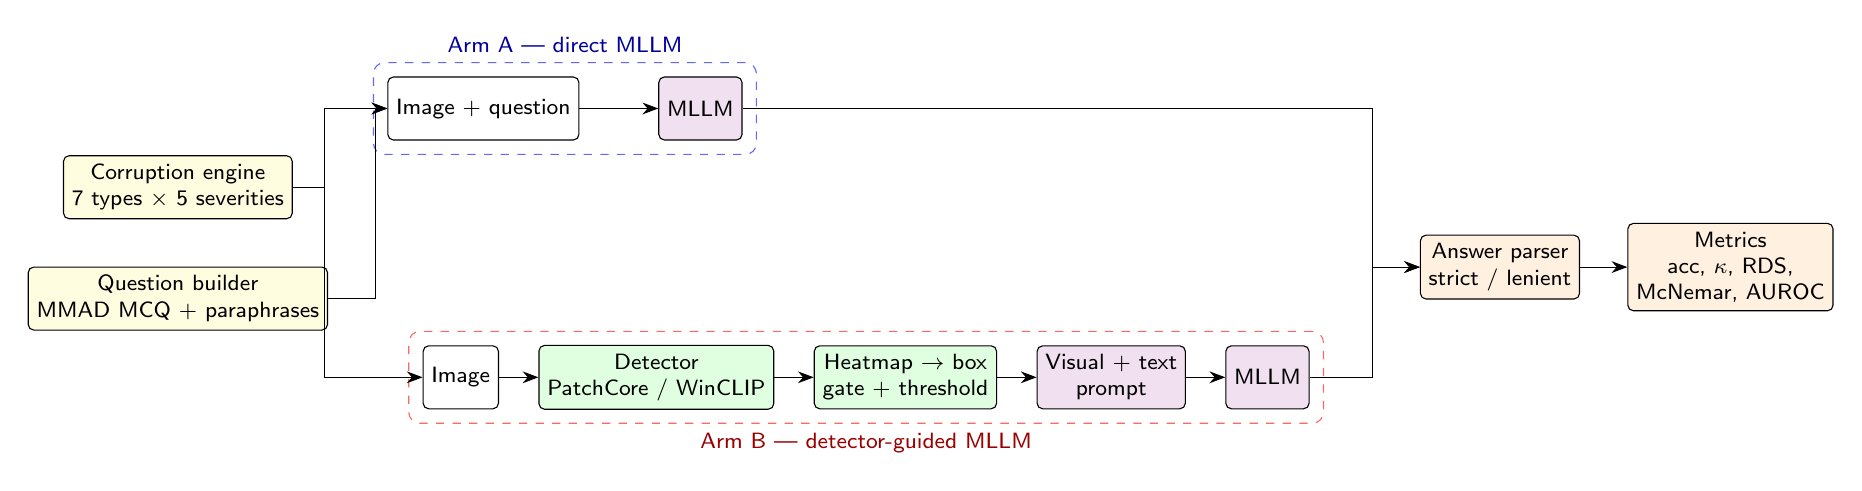
\begin{tikzpicture}[
  font=\sffamily\footnotesize, >={Stealth[length=2mm]},
  box/.style={draw, rounded corners=2pt, align=center, minimum height=8mm, inner sep=3pt, fill=white},
  src/.style={box, fill=yellow!12},
  det/.style={box, fill=green!12},
  llm/.style={box, fill=violet!12},
  evl/.style={box, fill=orange!12},
  arm/.style={draw, dashed, rounded corners=4pt, inner sep=5pt}]
  % inputs
  \node[src] (cor) {Corruption engine\\7 types $\times$ 5 severities};
  \node[src, below=6mm of cor] (qb) {Question builder\\MMAD MCQ + paraphrases};
  % arm A
  \node[box, right=12mm of cor, yshift=10mm] (a_in) {Image + question};
  \node[llm, right=10mm of a_in] (a_llm) {MLLM};
  % arm B
  \node[box, right=12mm of qb, yshift=-10mm] (b_img) {Image};
  \node[det, right=5mm of b_img] (b_det) {Detector\\PatchCore / WinCLIP};
  \node[det, right=5mm of b_det] (b_box) {Heatmap $\rightarrow$ box\\gate + threshold};
  \node[llm, right=5mm of b_box] (b_vp) {Visual + text\\prompt};
  \node[llm, right=5mm of b_vp] (b_llm) {MLLM};
  % outputs
  \node[evl, right=14mm of b_llm, yshift=14mm] (parse) {Answer parser\\strict / lenient};
  \node[evl, right=6mm of parse] (met) {Metrics\\acc, $\kappa$, RDS,\\McNemar, AUROC};
  % arm frames
  \begin{scope}[on background layer]
    \node[arm, draw=blue!60, fit=(a_in)(a_llm), label={[blue!60!black]above:\armA{} --- direct MLLM}] (fa) {};
    \node[arm, draw=red!60, fit=(b_img)(b_llm), label={[red!60!black]below:\armB{} --- detector-guided MLLM}] (fb) {};
  \end{scope}
  \draw[->] (cor.east) -- ++(4mm,0) |- (a_in.west);
  \draw[->] (cor.east) -- ++(4mm,0) |- (b_img.west);
  \draw[->] (qb.east) -- ++(6mm,0) |- (a_in.west);
  \draw[->] (a_in) -- (a_llm);
  \draw[->] (b_img) -- (b_det);
  \draw[->] (b_det) -- (b_box);
  \draw[->] (b_box) -- (b_vp);
  \draw[->] (b_vp) -- (b_llm);
  \draw[->] (a_llm.east) -| ($(parse.west)+(-6mm,0)$) -- (parse.west);
  \draw[->] (b_llm.east) -| ($(parse.west)+(-6mm,0)$) -- (parse.west);
  \draw[->] (parse) -- (met);
\end{tikzpicture}}
\caption{Study design. \armA{} gives the MLLM the image and question directly.
\armB{} first runs an unsupervised anomaly detector, converts its heatmap into a box,
and shows the MLLM where the detector points before it answers. Both arms receive
identical (optionally corrupted) images and questions, so they can be compared
question by question.}
\label{fig:pipeline}
\end{figure*}

% =============================================================================
\section{Related Work}

\textbf{MLLMs for industrial inspection.} MMAD~\cite{jiang2025mmad} defines seven
inspection subtasks and evaluates 1-shot MLLMs with a normal template image.
AnomalyGPT~\cite{gu2024anomalygpt} fine-tunes an LVLM with a learned anomaly
decoder and scores 36.5 on MMAD, below general-purpose models, which suggests
general visual-language competence matters more than narrow anomaly training for
MMAD's question types.

\textbf{Unsupervised anomaly detection.} PatchCore~\cite{roth2022patchcore} compares
mid-level patch features with a coreset memory of normal patches and gives
near-perfect localisation on MVTec-AD. WinCLIP~\cite{jeong2023winclip} scores image
windows against ``normal/damaged object'' prompts in CLIP~\cite{radford2021clip}
space, zero-shot or with a few normal shots (WinCLIP+). Both produce heatmaps but no
explanation, which is the complementarity \armB{} tries to exploit.

\textbf{Visual prompting.} Drawing a red circle steers CLIP's
attention~\cite{shtedritski2023red}, and Set-of-Mark~\cite{yang2023som} overlays
region marks to ground GPT-4V. Whether such marks help or \emph{mislead} small MLLMs
on fine-grained defects is the open question for \armB.

\textbf{Robustness.} Common-corruption benchmarks~\cite{hendrycks2019benchmarking}
show large accuracy drops for vision models; MMAD evaluates only clean captures.

\textbf{Small open MLLMs.} We evaluate Qwen2-VL/2.5-VL/3-VL~\cite{wang2024qwen2vl,
bai2025qwen25vl,qwen3vl}, SmolVLM~\cite{marafioti2025smolvlm}, Gemma~4~\cite{gemma4},
Moondream2~\cite{moondream2} and PaliGemma~2~\cite{steiner2024paligemma2}; larger
models are run in 4-bit NF4~\cite{dettmers2023qlora}.

% =============================================================================
\section{Experimental Setup}\label{sec:setup}

\textbf{Data.} MMAD's 8{,}366 images and 39{,}672 questions carry nine subtask labels.
Following the MMAD paper, \emph{Object Analysis}, \emph{Object Structure} and
\emph{Object Details} are folded into one ``Object Analysis'' column when reporting
the seven-task average, and the seven-task average is the unweighted column mean
(this reproduces 20 of the 21 printed MMAD rows exactly). Anomaly discrimination is
reported as MMAD's balanced accuracy (mean of normal- and abnormal-class accuracy).

\textbf{Sampling.} Unless stated otherwise, questions are drawn stratified by
subtask (equal share per subtask, remainder at random) with seed 42. Phase~1 and
Phase~4 use $N{=}2{,}500$; the robustness study uses 5{,}000 questions.

\textbf{Inference.} Zero-shot, greedy decoding, 4--8 new tokens, the question and
lettered options followed by ``Answer with the letter of the correct option\ldots''.
Qwen images are limited to $512{\times}28{\times}28$ pixels. Hardware: RTX 4060 Laptop
(8.19\,GB), PyTorch 2.6 / CUDA 12.4.

\textbf{Metrics.} Accuracy with Wilson 95\,\% intervals~\cite{wilson1927}; Cohen's
$\kappa$~\cite{cohen1960kappa} between predicted and true letters; the robustness
degradation slope $\mathrm{RDS}(s) = (\mathrm{Acc}_{\text{clean}} -
\mathrm{Acc}_{s})/s$ in points per severity level; paired comparisons with the exact
McNemar test~\cite{mcnemar1947}; for detectors, image AUROC, pixel AUROC and box IoU
against MMAD's ground-truth masks. At $n{\approx}278$ per subtask the 95\,\%
half-width is about $\pm$5.8\pp, and at $n{=}2{,}500$ about $\pm$1.8\pp; smaller
differences are not claimed as effects.

% =============================================================================
\section{Results}

\subsection{Clean baseline (Phases 0--1)}\label{sec:clean}

Qwen3-VL-2B (FP16; 4.26\,GB allocated after loading, 4.82\,GB peak) answers 1{,}780 of 2{,}500 questions correctly:
71.2\,\% [69.4, 72.9], $\kappa{=}0.615$, 0.16\,s per question (6.2 questions/s), with
100\,\% of outputs parseable. Table~\ref{tab:clean} and Fig.~\ref{fig:clean} show
the profile: object-level questions are easy (Object Classification 94.9\,\%), while
the two questions an inspector cares most about, \emph{which defect}
(Defect Classification 40.8\,\%) and \emph{where} (Defect Localization 47.5\,\%),
are the weakest. MVTec-LOCO, whose anomalies are logical rather than visual, is the
hardest source (61.6\,\%).

With MMAD's official evaluation code in its 1-shot setting (one normal template),
Qwen3-VL-2B reaches 70.8\,\% on 18{,}651 questions from 3{,}800 images
(MVTec-AD images via DS-MVTec 78.3\,\%, VisA 75.8\,\%, MVTec-LOCO 60.9\,\%). GoodsAD is
not yet covered, so this is not a full-benchmark number \todo{finish GoodsAD}.

\begin{table}[t]
\centering
\caption{Qwen3-VL-2B zero-shot, $N{=}2{,}500$ (Phase~1).}
\label{tab:clean}
\footnotesize
\begin{tabular}{@{}lrr@{\hspace{10pt}}lrr@{}}
\toprule
Subtask & $n$ & Acc & Source & $n$ & Acc \\
\midrule
Object Classif. & 277 & 94.9 & DS-MVTec & 497 & 77.5 \\
Object Analysis & 277 & 82.3 & VisA & 787 & 74.6 \\
Defect Analysis & 278 & 82.0 & GoodsAD & 716 & 69.8 \\
Object Structure & 277 & 81.2 & MVTec-LOCO & 500 & 61.6 \\
Object Details & 277 & 79.8 & & & \\
Defect Descr. & 277 & 71.1 & & & \\
Anomaly Det. & 282 & 61.3 & & & \\
Defect Local. & 278 & 47.5 & & & \\
Defect Classif. & 277 & 40.8 & & & \\
\midrule
\textbf{All} & 2500 & \textbf{71.2} & & & \\
\bottomrule
\end{tabular}
\end{table}

\begin{figure}[t]
\centering
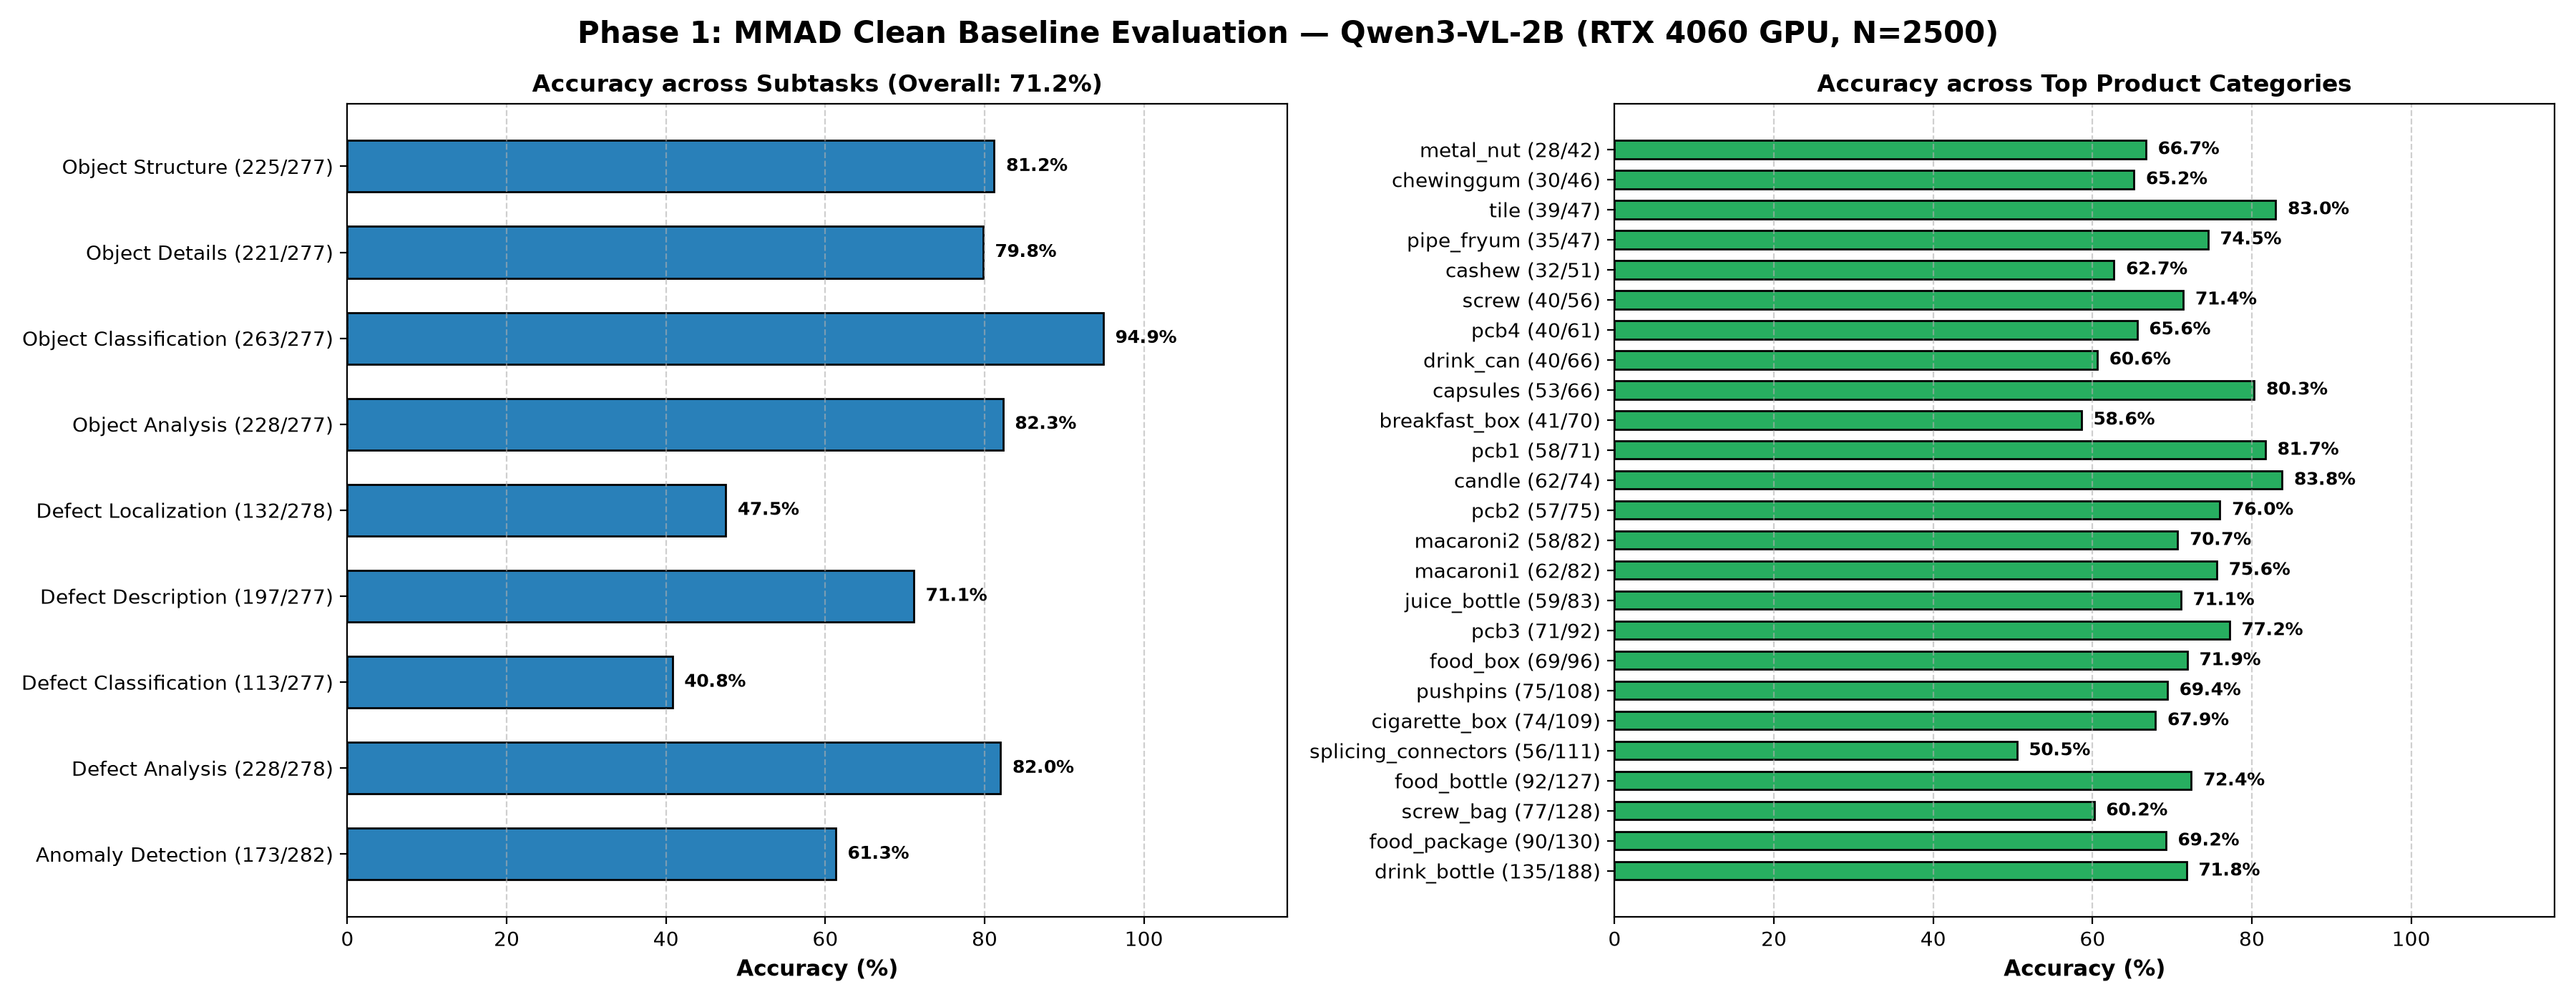
\includegraphics[width=\columnwidth]{phase1_subtask_accuracy.png}
\caption{Phase~1 accuracy by subtask (Qwen3-VL-2B, zero-shot, $N{=}2{,}500$).}
\label{fig:clean}
\end{figure}

\subsection{Model zoo and deployment envelope (Phase 4)}\label{sec:zoo}

Table~\ref{tab:zoo} evaluates ten open models on the same 2{,}500 questions
(Phase~1's draw differs from the Phase-4 draw by four Anomaly Detection questions).
Three observations:

\emph{Small open models reach the upper half of the MMAD leaderboard.} Under MMAD's
seven-task protocol (Fig.~\ref{fig:leader}), Qwen3-VL-8B (4-bit) scores 70.5 and
Qwen3-VL-2B 68.4, above every open model $\le$34\,B in the MMAD paper and on par with
Gemini-1.5-flash (68.9) and Claude-3.5-sonnet (68.4). The 8B and 2B models are not
separable from each other at this sample size (72.2 vs 71.2 on nine tasks).
These comparisons are 0-shot against the paper's 1-shot; MMAD's own 0/1-shot
ablation moves models by $-1.3$ to $+1.9$ points (Fig.~\ref{fig:shot}), so
differences below about two points are not meaningful.

\emph{Defect localisation separates encoder families.} On Defect Localization
(Fig.~\ref{fig:loc}), Qwen dynamic-resolution encoders score 47.5--56.0 and
Moondream2 59.2, while both Gemma~4 models (31.4, 26.4) and SmolVLM (33.2, 29.6)
sit near the 25\,\% chance level; at matched 4.4\,B scale Qwen3-VL-4B beats
Gemma-4-E4B by 20.2\pp. Qwen3-VL-8B (56.0) and Moondream2 (59.2) are statistically
indistinguishable from GPT-4o (55.6) at $n{\approx}278$ ($\pm$5.8\pp).

\emph{Deployability is not monotone in size} (Fig.~\ref{fig:env}). The fastest model
(Qwen3-VL-2B, 6.2\,q/s) is also among the most accurate; NF4 quantisation puts
Qwen3-VL-4B in 3.1\,GB. Below 1\,B parameters accuracy collapses (SmolVLM-500M
45.7\,\%, SmolVLM-256M 32.6\,\%). PaliGemma~2 (8.2\,\%) is a \emph{pre-trained},
not instruction-tuned, checkpoint that does not produce option letters; it is a
format failure rather than a capability measurement and should be dropped or
re-run with its mix checkpoint \todo{decide}.

\begin{table*}[t]
\centering
\caption{Ten open models on the same 2{,}500 MMAD questions (0-shot, RTX~4060 Laptop).
MMAD-7 = unweighted mean of MMAD's seven task columns (balanced anomaly
discrimination). DL = Defect Localization. Latency per question, batch size 1.}
\label{tab:zoo}
\footnotesize
\resizebox{\textwidth}{!}{%
\begin{tabular}{@{}lrlrrrrrrr@{}}
\toprule
Model & Params (B) & Precision & VRAM (GB) & Acc (9 tasks) & $\kappa$ & MMAD-7 & DL & Latency (s) & q/s \\
\midrule
Qwen3-VL-8B       & 8.20 & NF4  & 6.73 & \textbf{72.16} & \textbf{0.627} & \textbf{70.51} & 55.96 & 0.32 & 3.1 \\
Qwen3-VL-2B       & 2.20 & FP16 & 4.82 & 71.20 & 0.615 & 68.40 & 47.50 & \textbf{0.16} & \textbf{6.2} \\
Qwen3-VL-4B       & 4.40 & NF4  & 3.06 & 68.80 & 0.582 & 66.72 & 51.62 & 0.19 & 5.3 \\
Qwen2.5-VL-3B     & 3.10 & FP16 & 5.86 & 67.68 & 0.574 & 65.51 & 51.26 & 0.22 & 4.5 \\
Moondream2        & 1.80 & FP16 & 2.10 & 67.56 & 0.567 & 66.13 & \textbf{59.21} & 0.45 & 2.2 \\
Gemma-4-E4B       & 4.40 & NF4  & 3.32 & 65.60 & 0.540 & 62.58 & 31.41 & 0.85 & 1.2 \\
Gemma-4-E2B       & 2.30 & FP16 & 4.65 & 60.92 & 0.476 & 58.80 & 26.35 & 0.34 & 3.0 \\
SmolVLM-500M      & 0.50 & FP16 & 1.11 & 45.72 & 0.277 & 43.43 & 33.21 & 0.46 & 2.2 \\
SmolVLM-256M      & 0.26 & FP16 & \textbf{0.85} & 32.56 & 0.123 & 32.66 & 29.60 & 0.44 & 2.3 \\
PaliGemma2-3B (pt)& 3.00 & FP16 & 5.80 & 8.20 & $-$0.076 & 7.91 & 10.11 & 0.21 & 4.7 \\
\midrule
\multicolumn{6}{@{}l}{\emph{MMAD paper (1-shot): GPT-4o / InternVL2-76B / Claude-3.5-sonnet}} & 74.92 / 70.75 / 68.36 & 55.62 / 56.66 / 48.81 & -- & -- \\
\bottomrule
\end{tabular}}
\end{table*}

\begin{figure}[t]
\centering
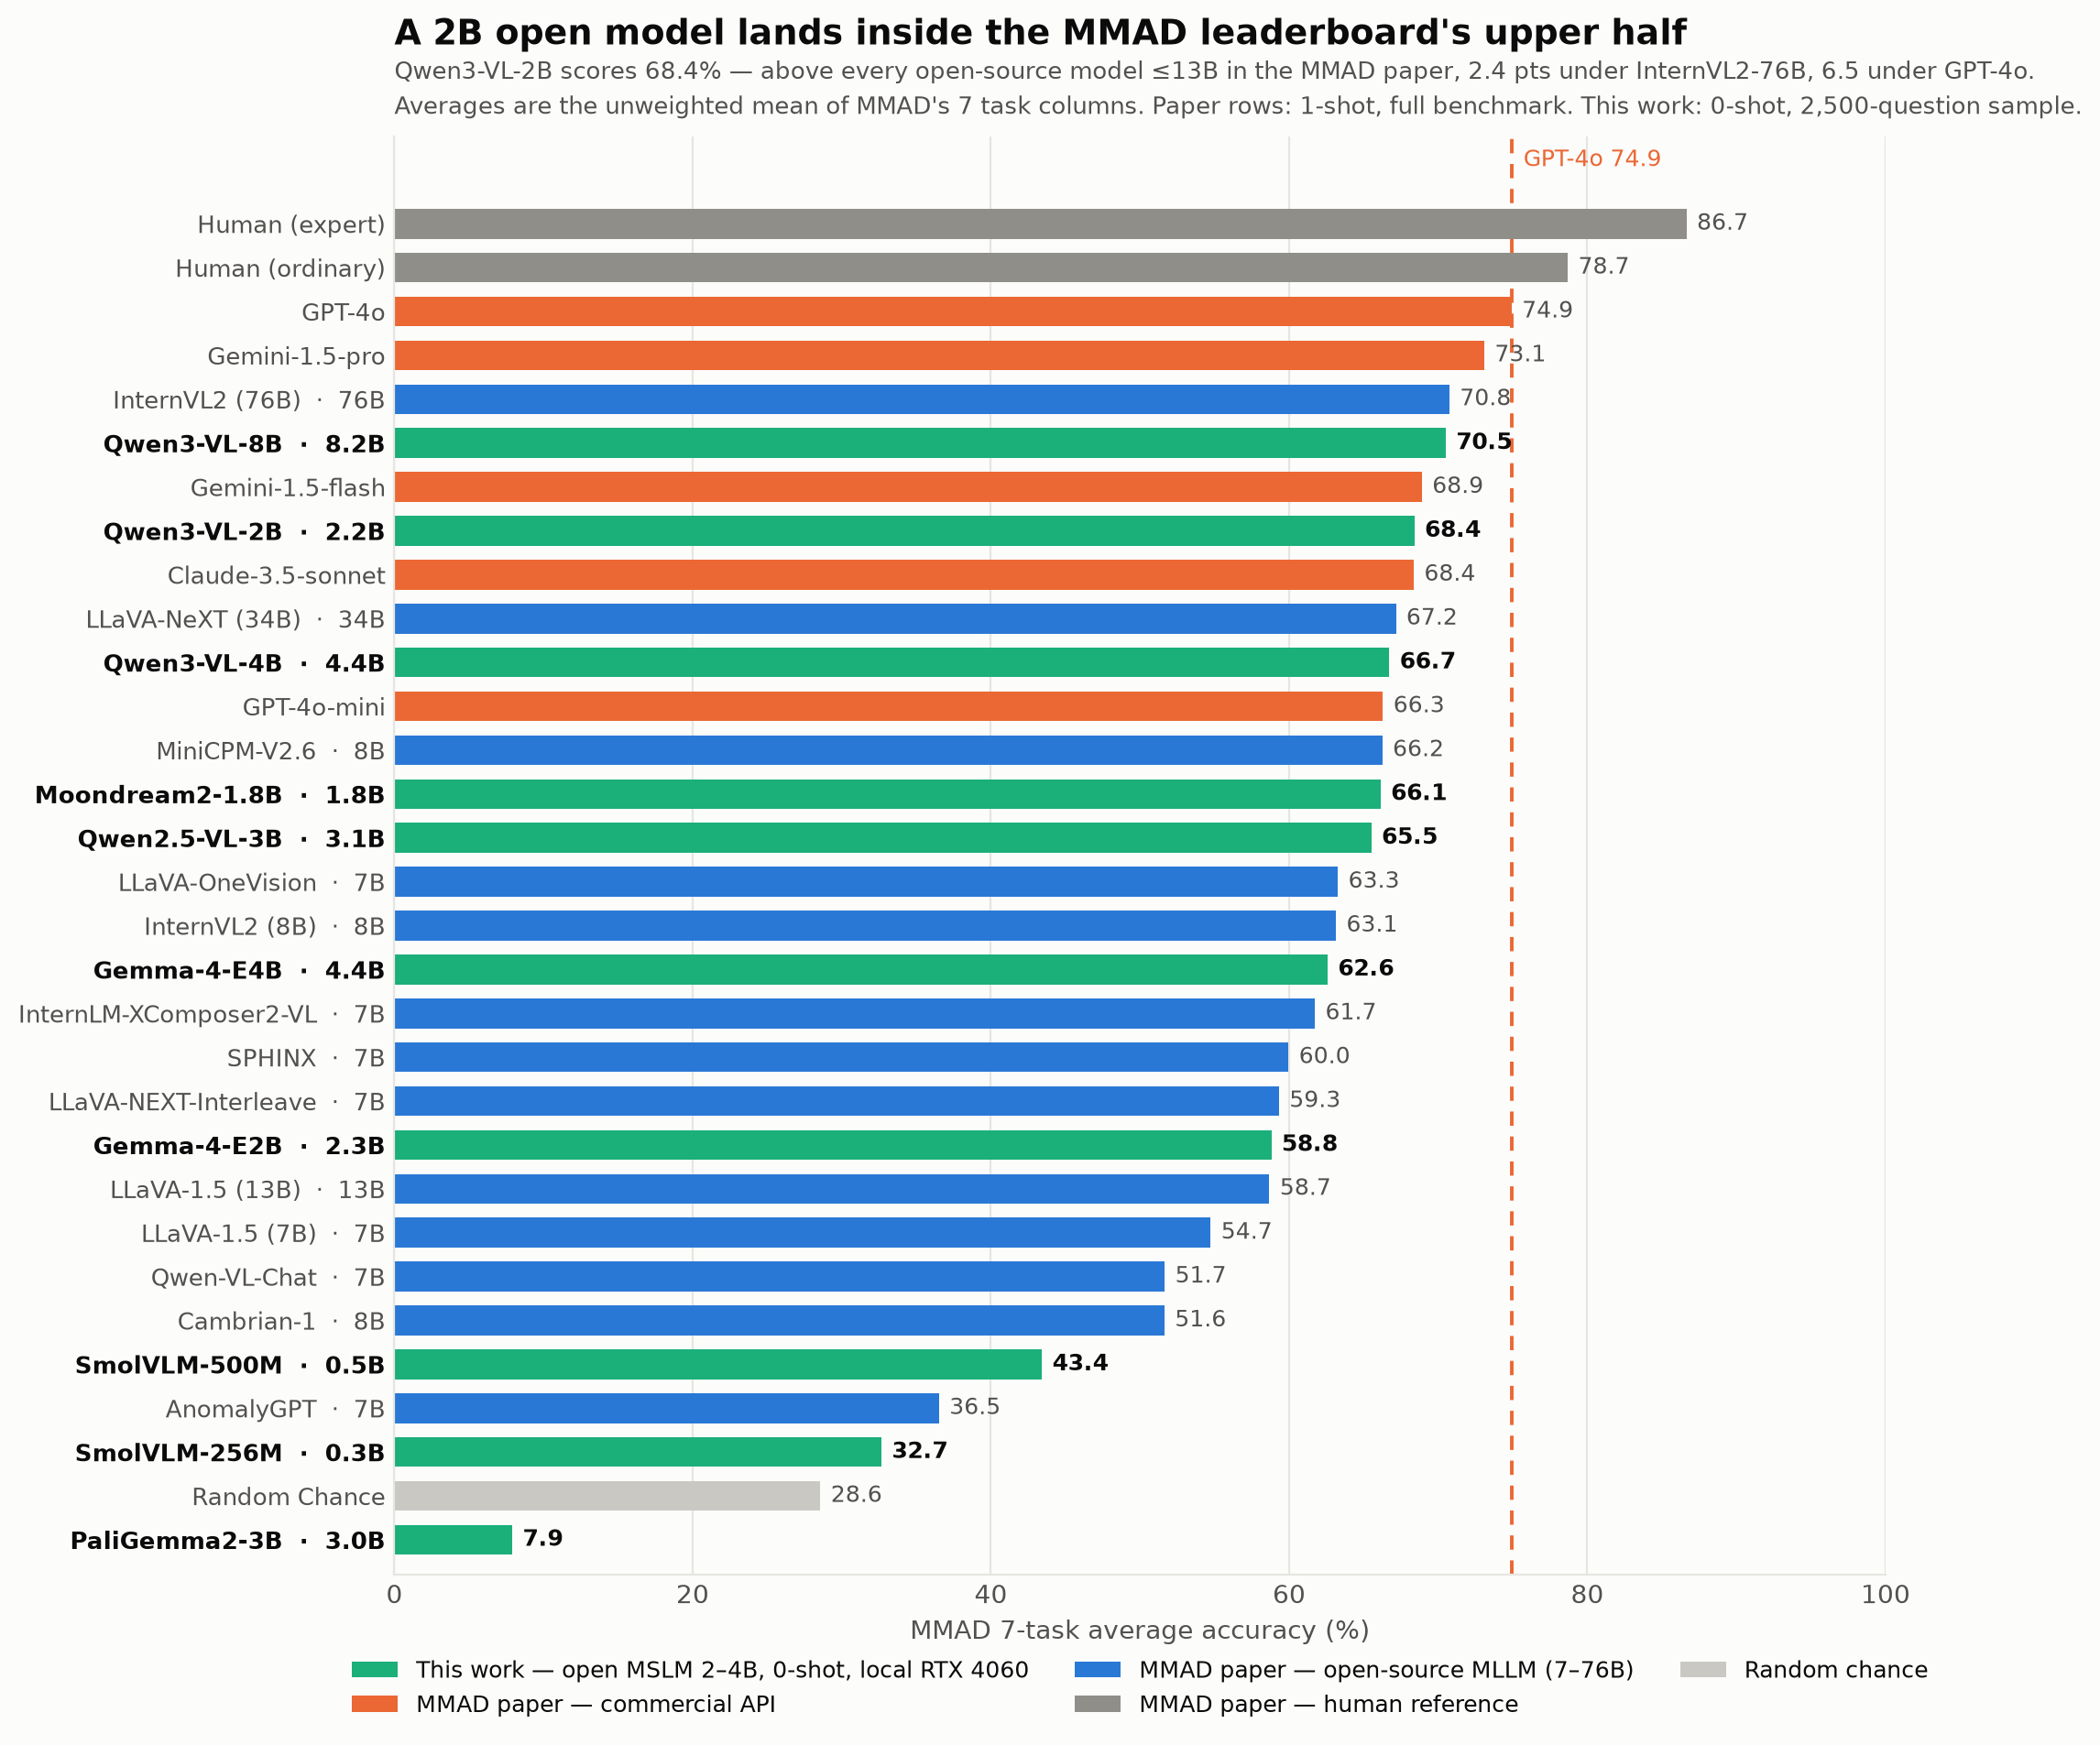
\includegraphics[width=\columnwidth]{fig1_overall_leaderboard.png}
\caption{Our models (green, 0-shot, 2{,}500 questions) placed on the MMAD
leaderboard (1-shot, full benchmark) by MMAD seven-task average.}
\label{fig:leader}
\end{figure}

\begin{figure}[t]
\centering
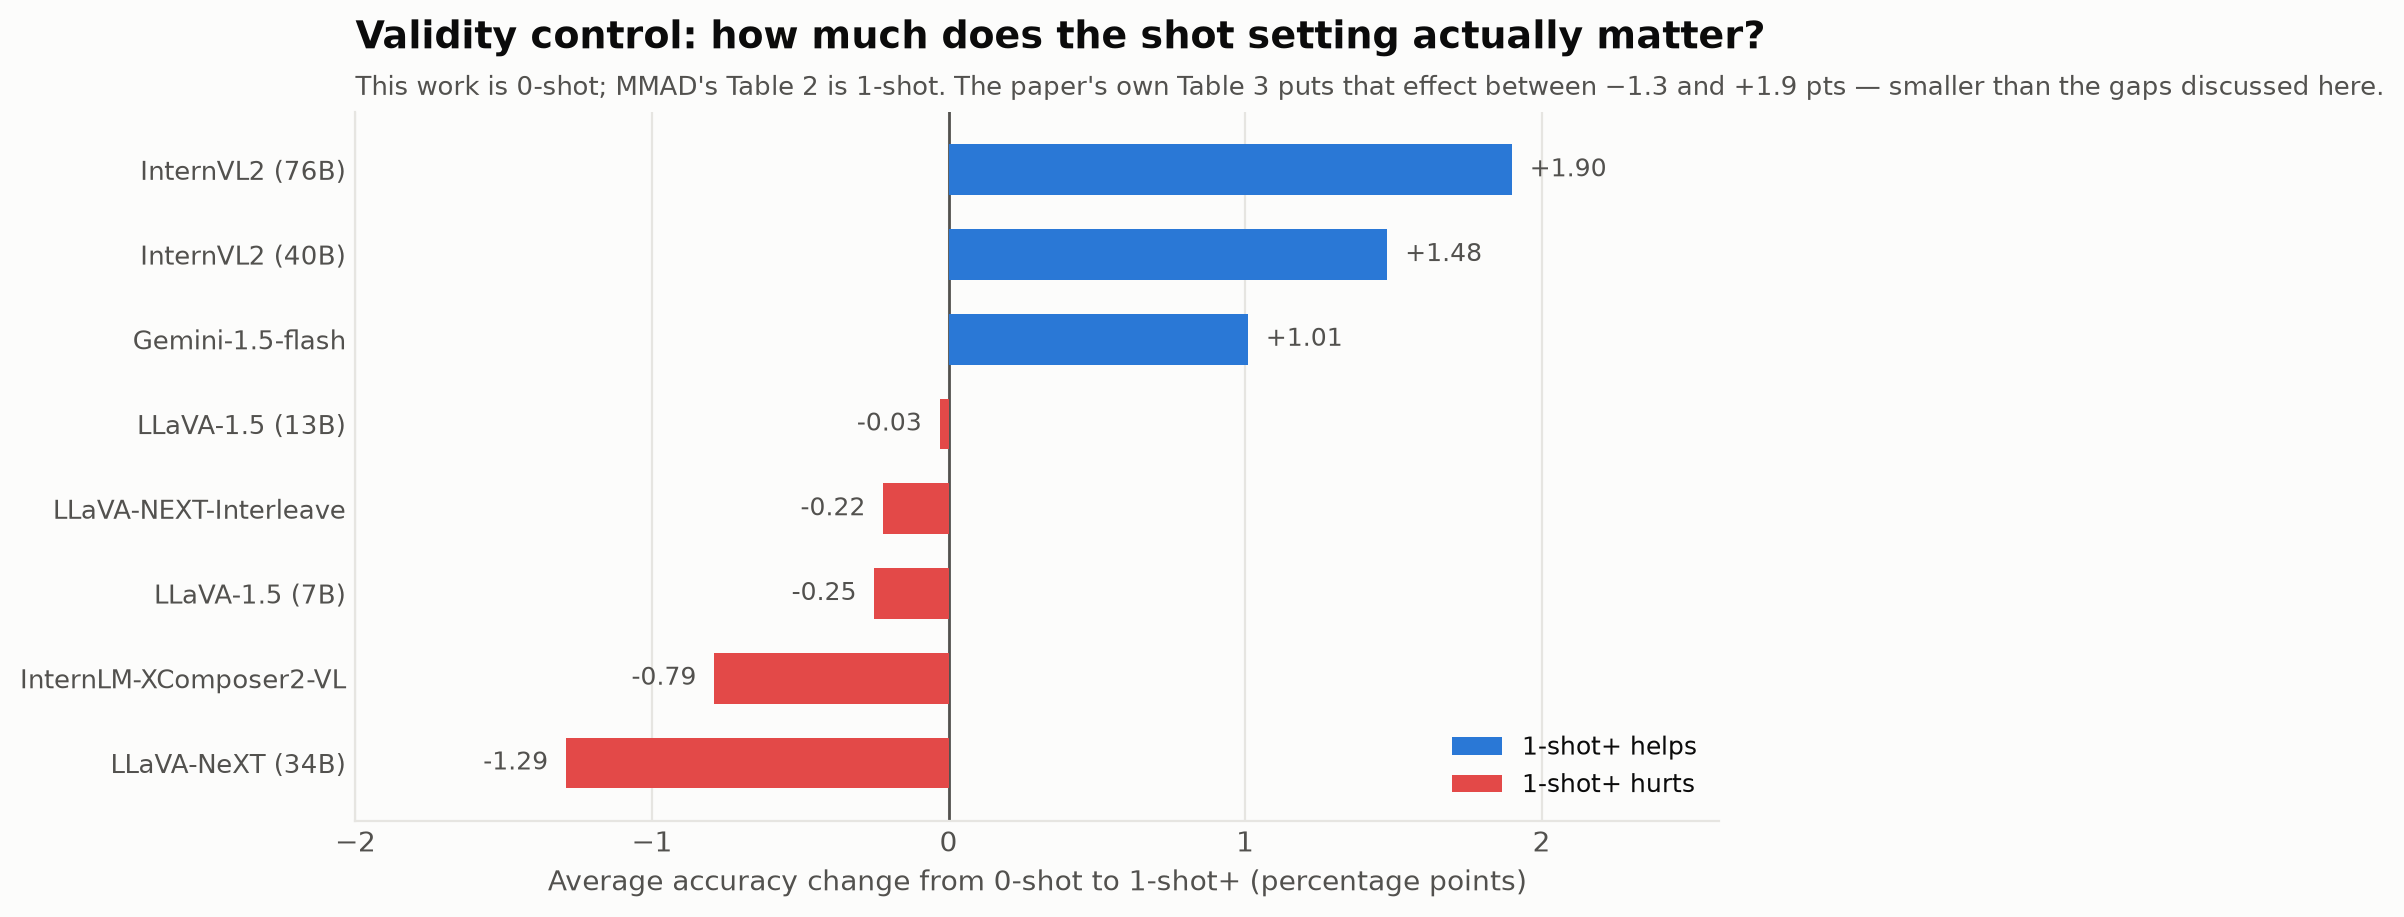
\includegraphics[width=\columnwidth]{fig7_shot_setting_control.png}
\caption{Validity control from the MMAD paper's own ablation: moving from 0-shot to
1-shot changes model averages by $-1.3$ to $+1.9$ points.}
\label{fig:shot}
\end{figure}

\begin{figure}[t]
\centering
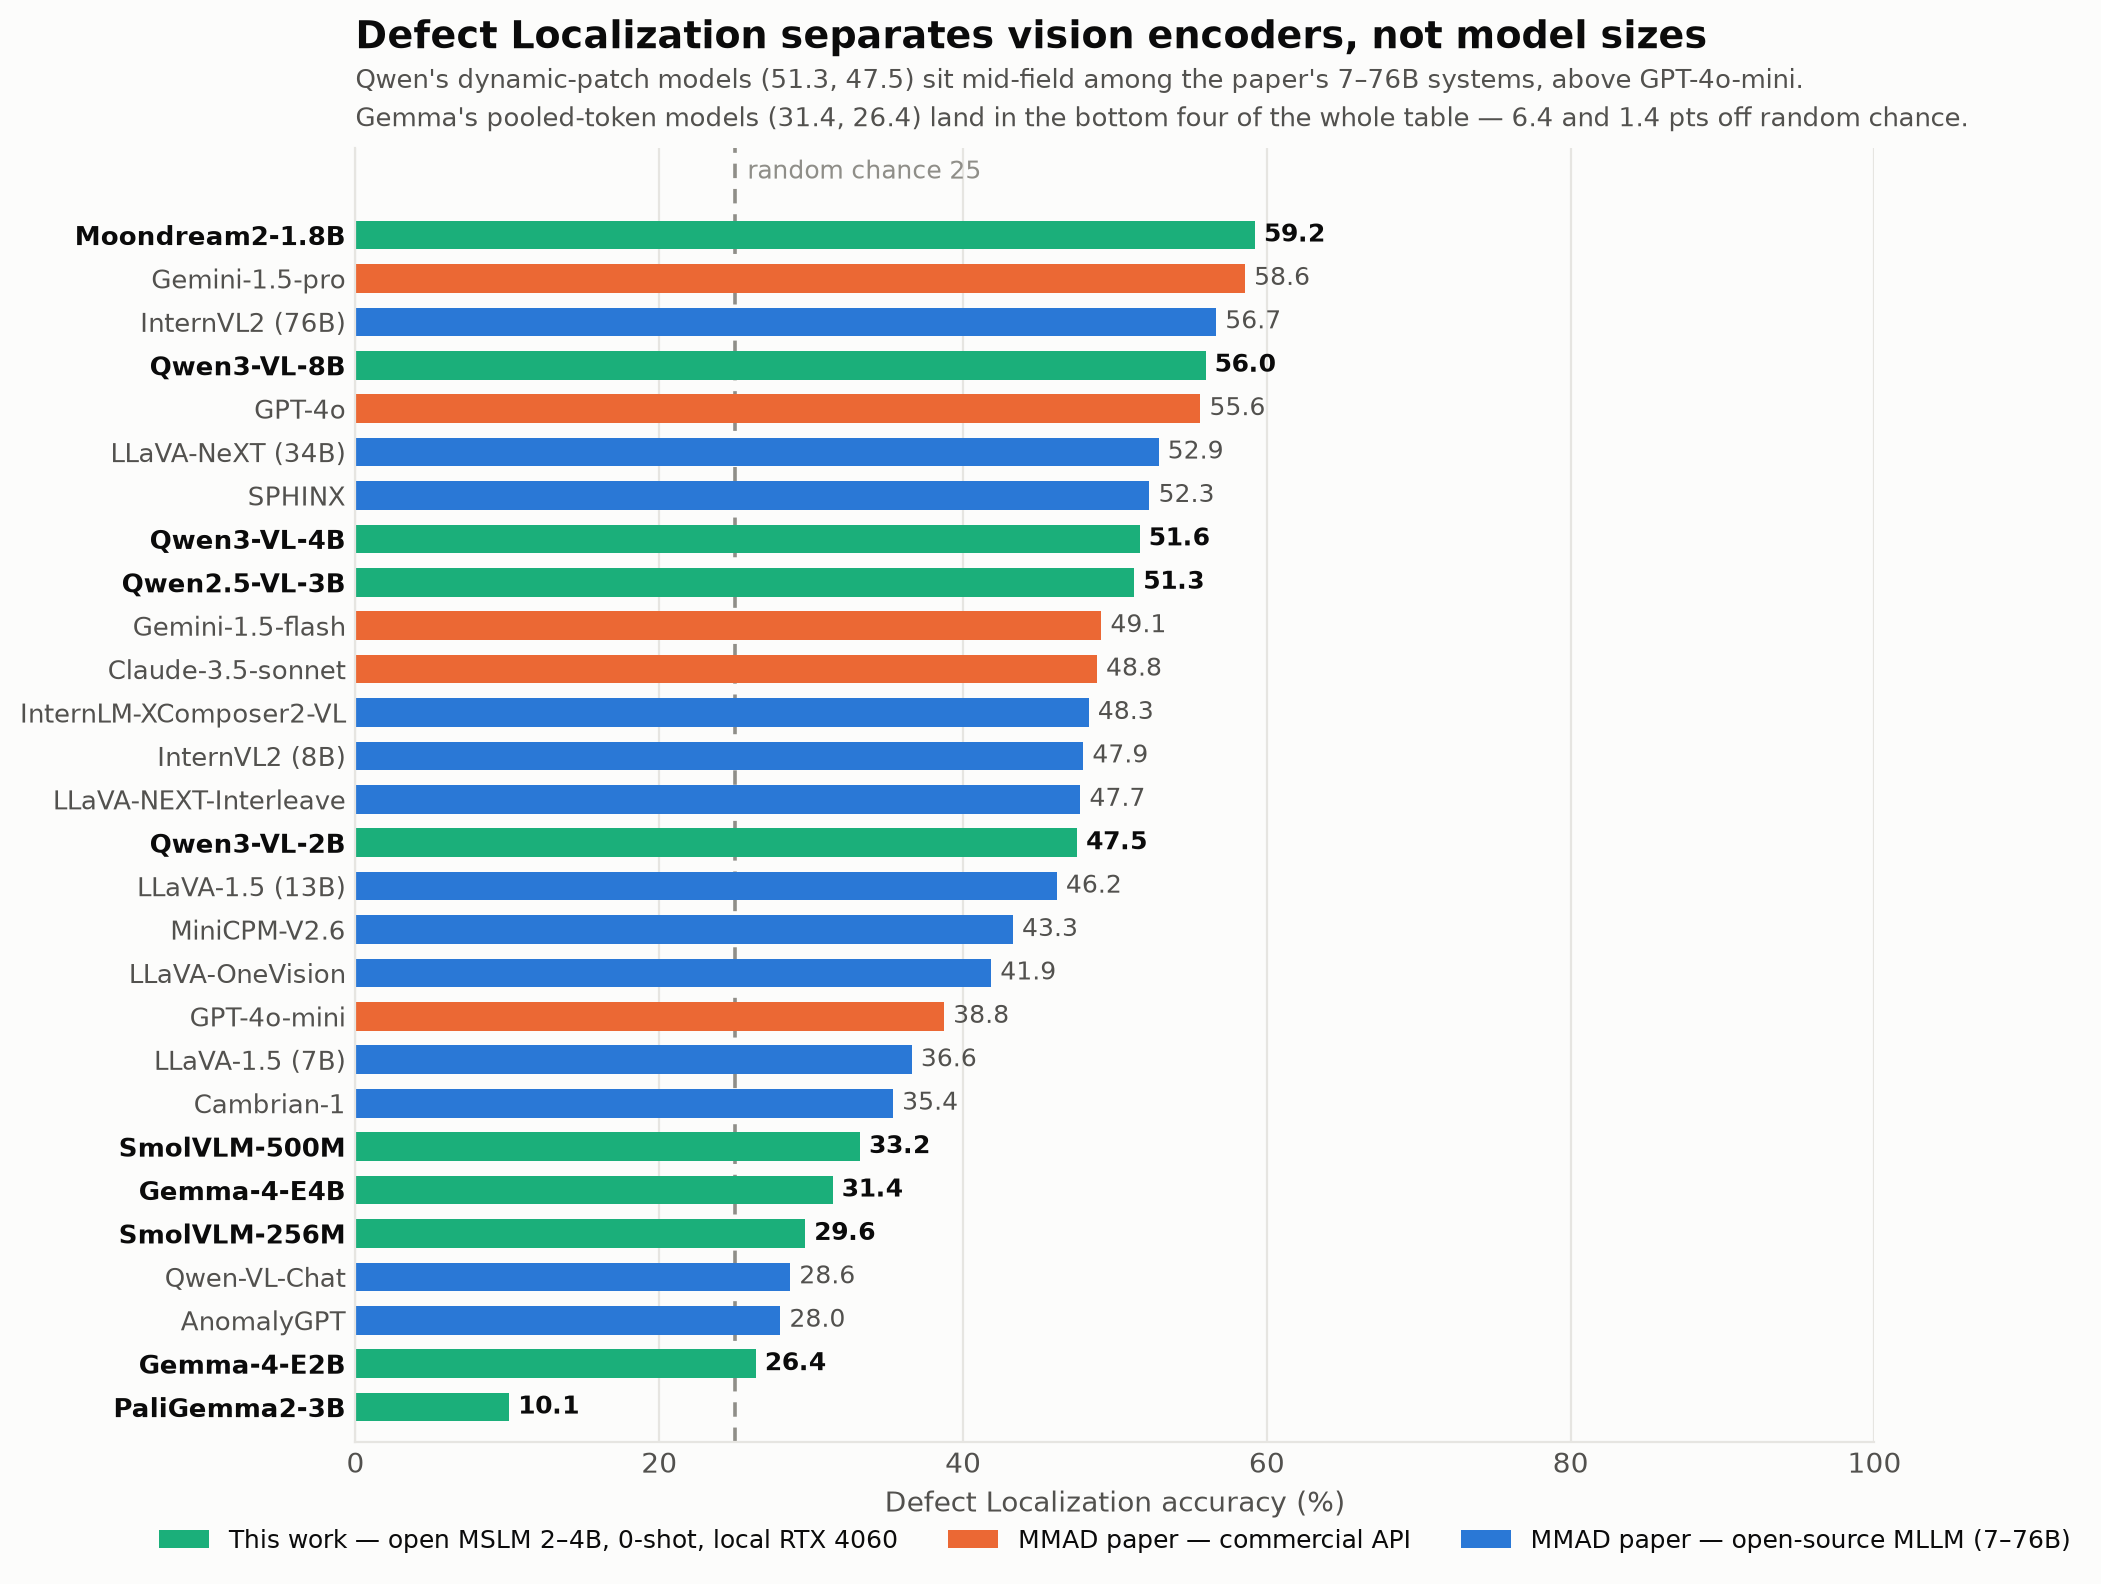
\includegraphics[width=\columnwidth]{fig5_defect_localization_gap.png}
\caption{Defect Localization across all models. Gemma~4 and SmolVLM, which pool
visual tokens aggressively, fall near chance. (Figure subtitle predates the 8B and
Moondream2 runs \todo{regenerate caption text in figure}.)}
\label{fig:loc}
\end{figure}

\begin{figure*}[t]
\centering
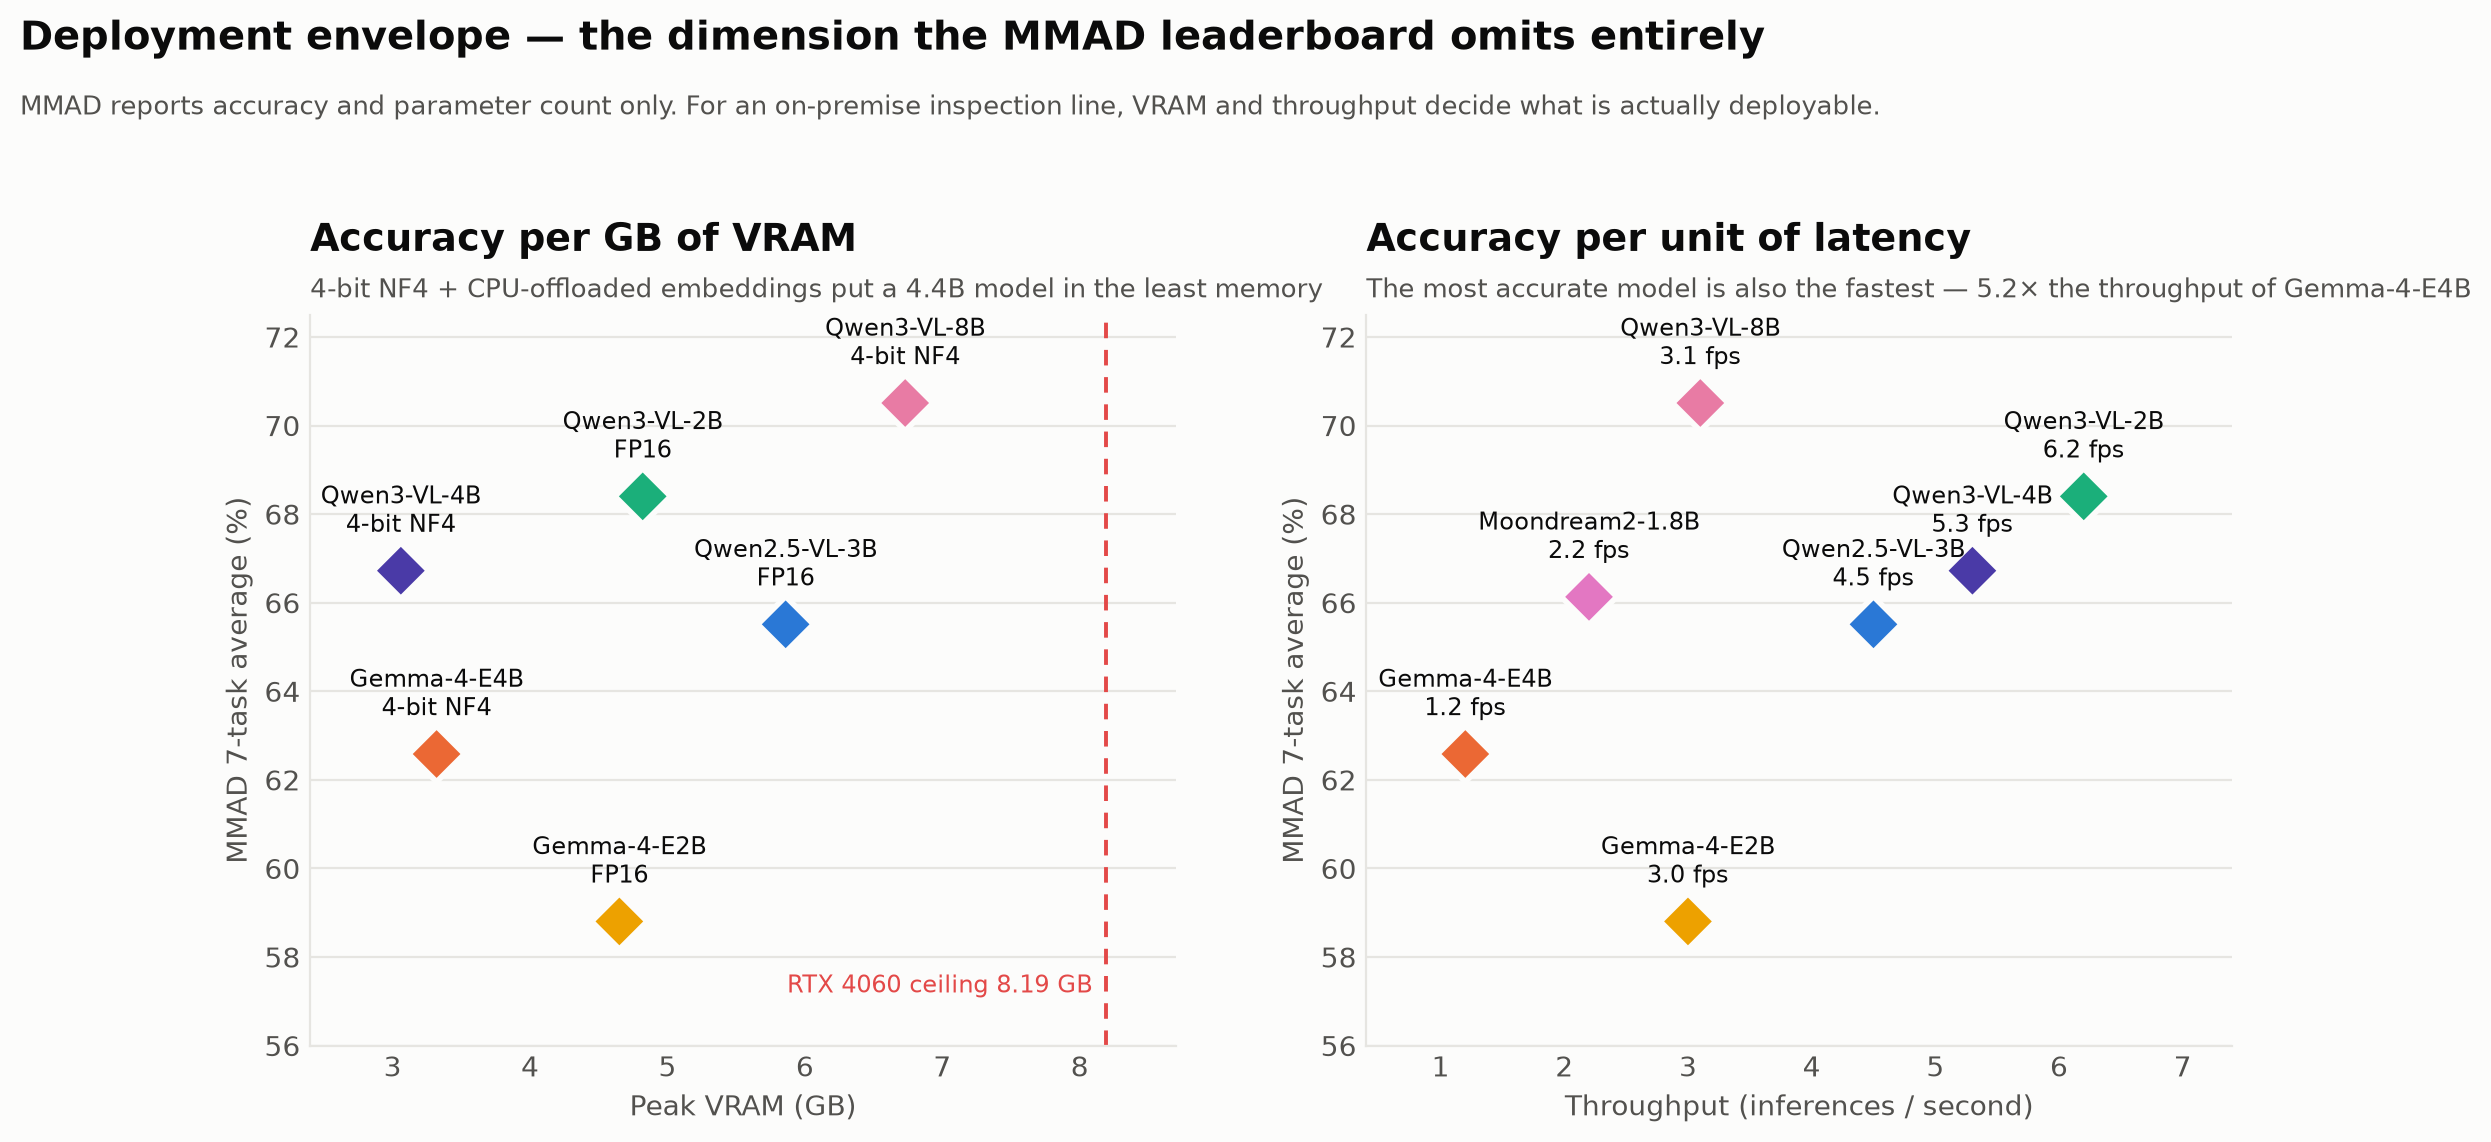
\includegraphics[width=0.49\textwidth]{fig8_deployment_envelope.png}\hfill
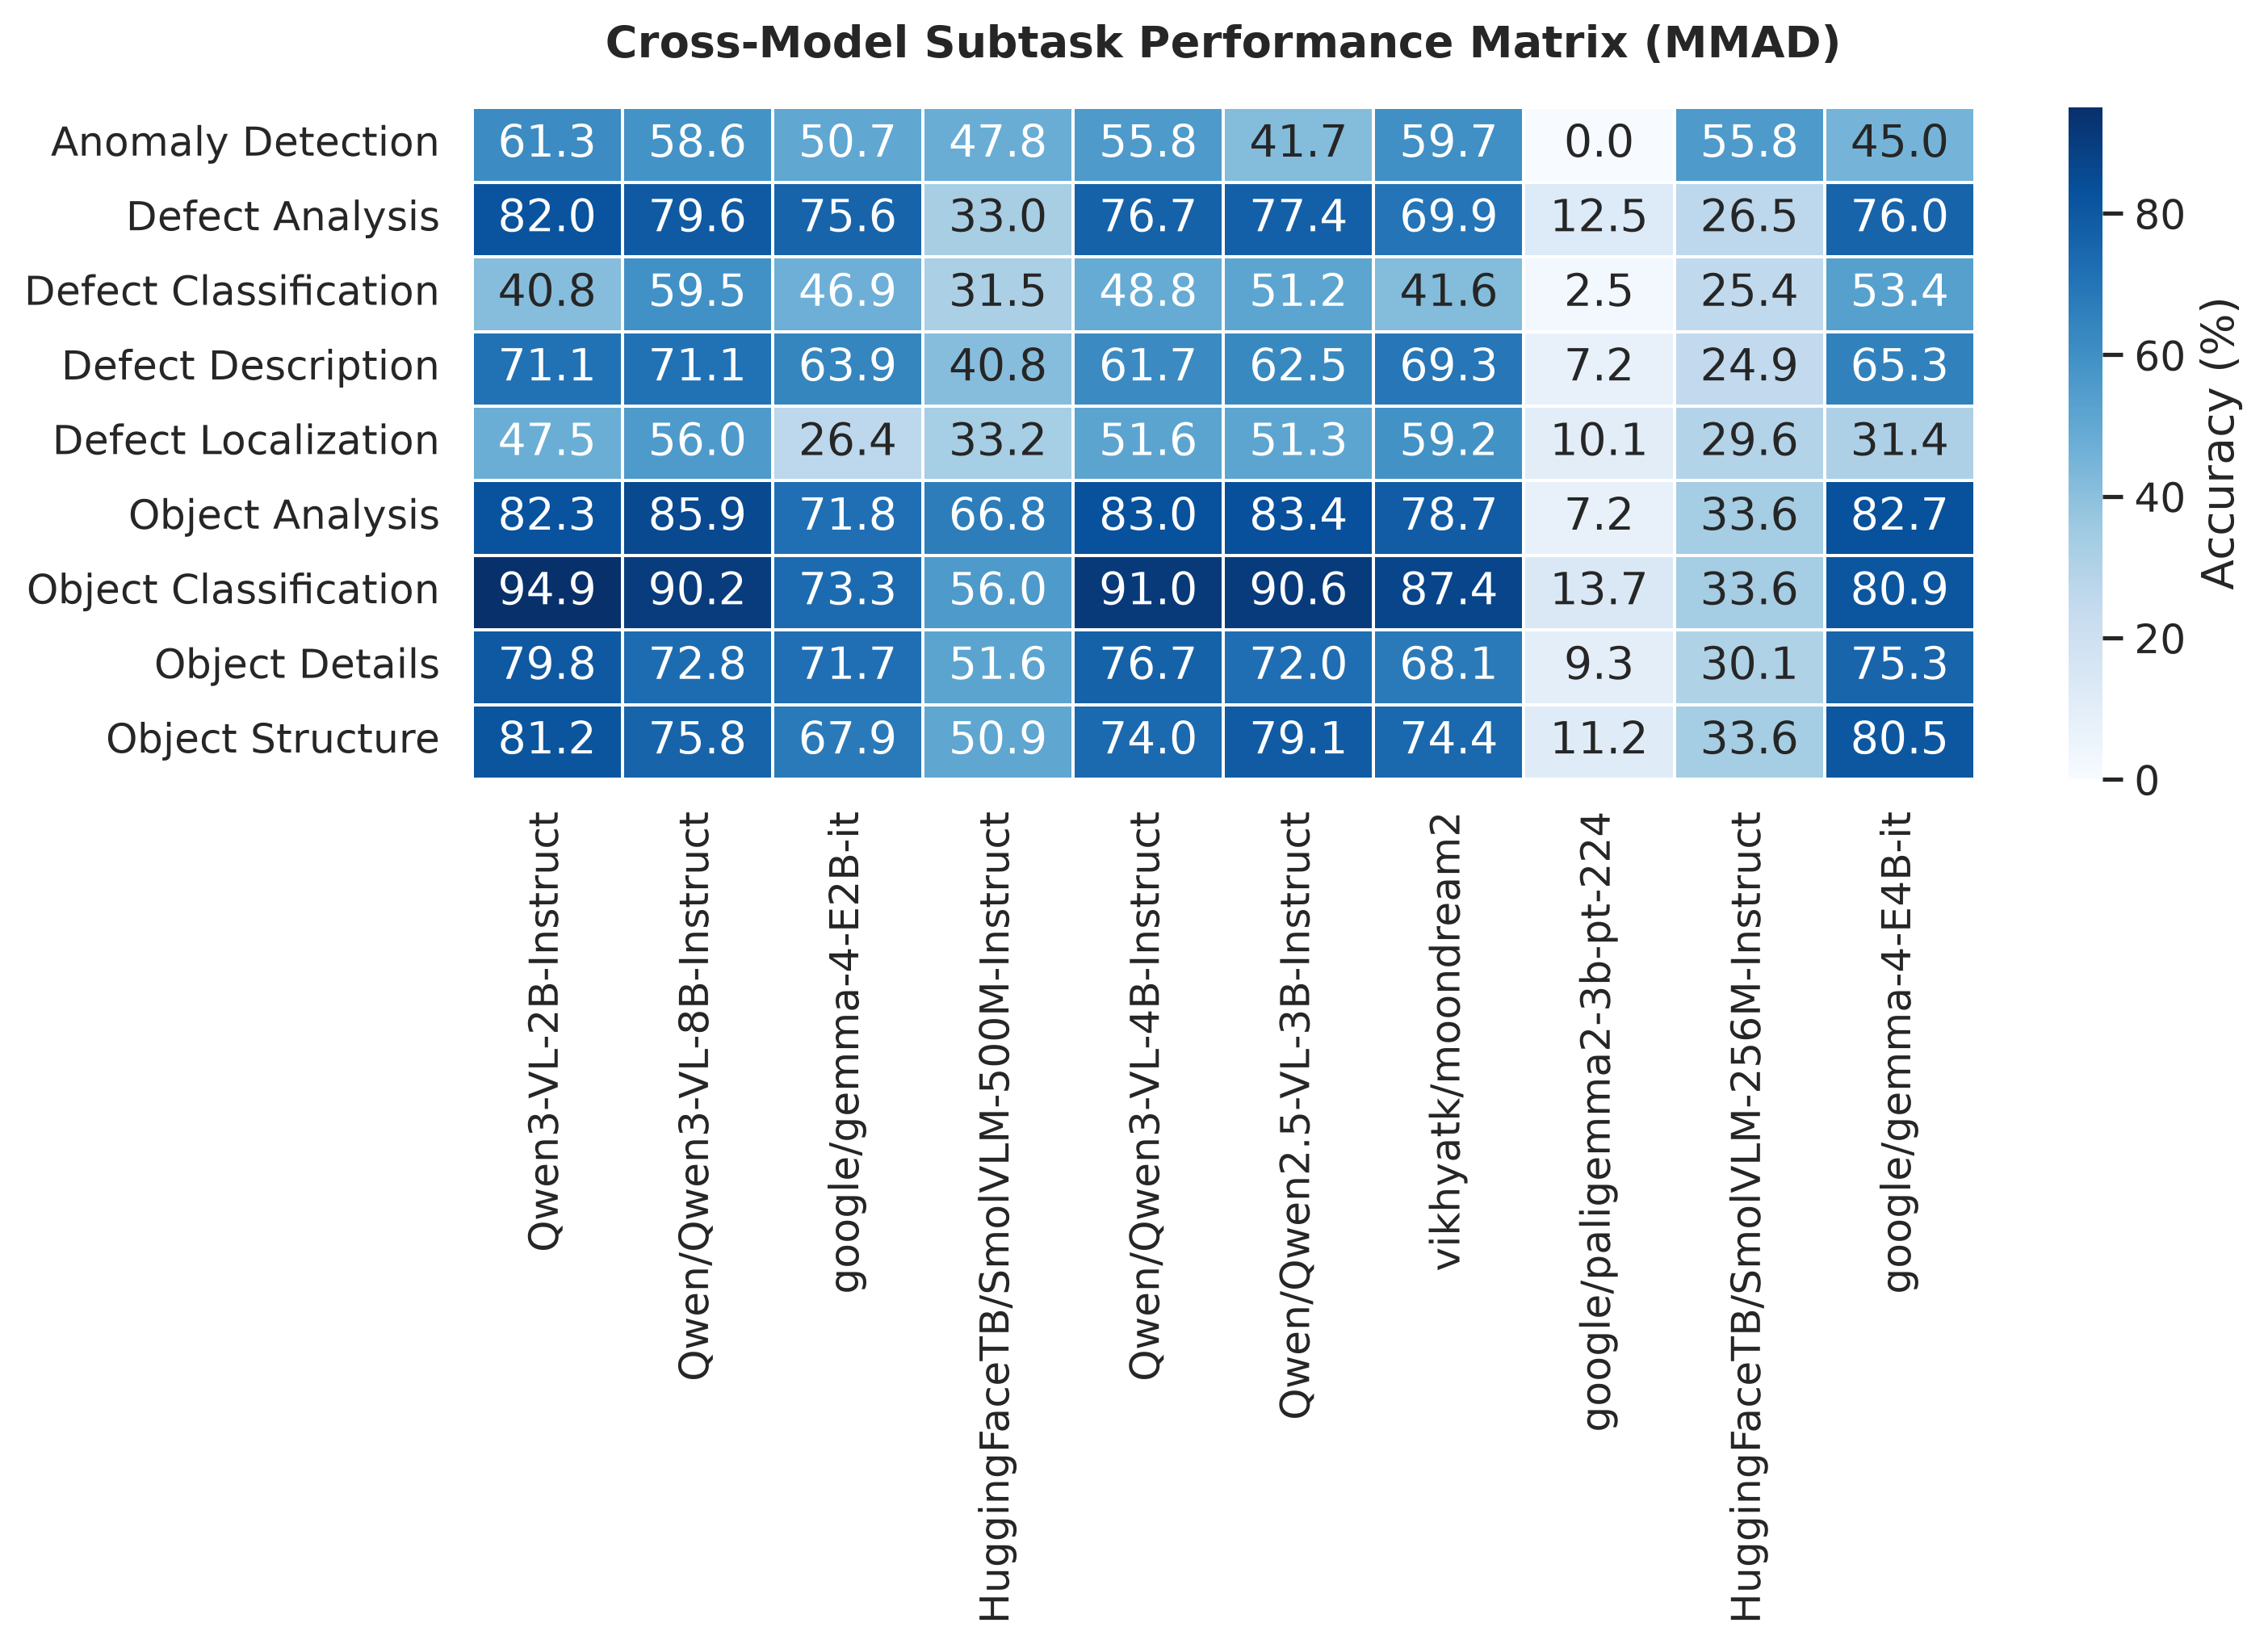
\includegraphics[width=0.49\textwidth]{phase4_subtask_accuracy_heatmap.png}
\caption{Left: accuracy against peak VRAM and throughput. Right: subtask accuracy
for all ten models (nine MMAD subtask labels).}
\label{fig:env}
\end{figure*}

\subsection{Robustness to factory-floor corruptions (Phases 2--3)}\label{sec:robust}

\textbf{Large-scale study.} Qwen3-VL-2B was evaluated on 5{,}000 questions in five
conditions (25{,}000 inferences): clean, severity-4 motion blur and severity-4
Gaussian noise, each also after test-time image restoration (TTA-IR: unsharp masking
for blur, bilateral filtering for noise). Table~\ref{tab:robust} and
Fig.~\ref{fig:robust} give the results.

The overall drop is modest (69.9 $\rightarrow$ 66.1 under blur, 66.6 under noise),
but it hides large opposite movements. Object-level subtasks collapse under blur
(Object Classification $-$19.4\pp, Object Analysis $-$17.5\pp, Object Structure
$-$13.7\pp), while Defect Classification \emph{rises} by 14.8\pp{} and Defect
Analysis by 9.2\pp. We do not read the rises as robustness: a blurred image is more
likely to be judged defective, which helps questions whose premise is that a defect
exists. This interpretation still needs a prediction-distribution check
\todo{confusion analysis per subtask}.

TTA-IR does not help overall ($-$0.3\pp{} on blur, $+$0.04\pp{} on noise). Its only
notable gain is Defect Localization under blur ($+$3.4\pp), within the per-subtask
noise band.

\textbf{Severity sweep (small).} A 7-corruption $\times$ 5-severity sweep with 45
questions per cell gave motion blur the steepest slope ($\mathrm{RDS}(5){=}1.78$\pp
per level) but curves that are not monotone in severity; at $n{=}45$ ($\pm$13\pp)
this sweep can rank corruptions only very coarsely and must be repeated at scale.

\textbf{Prompt-level mitigation.} A defect-anchored reasoning prompt (DAR) reduced
accuracy in all six corruption/severity cells of the small mitigation study
($-$4.4 to $-$15.6\pp, $n{=}45$ each), and TTA-IR changed accuracy by 0 to
$-$4.4\pp. The recovery-rate metric used there is undefined when corruption does not
lower accuracy, which happened in 5 of 6 cells; it is not reported.

\begin{table}[t]
\centering
\caption{Robustness at scale: Qwen3-VL-2B, 5{,}000 questions, severity~4.}
\label{tab:robust}
\footnotesize
\begin{tabular}{@{}lrrrrr@{}}
\toprule
Subtask & Clean & Blur & +TTA & Noise & +TTA \\
\midrule
Object Classif.  & 89.2 & 69.8 & 66.3 & 77.6 & 78.8 \\
Object Structure & 84.3 & 70.6 & 70.1 & 77.5 & 76.8 \\
Object Analysis  & 82.5 & 65.1 & 62.7 & 67.6 & 67.0 \\
Defect Analysis  & 76.9 & 86.1 & 86.9 & 87.4 & 87.8 \\
Object Details   & 74.1 & 62.3 & 62.2 & 67.2 & 69.0 \\
Defect Descr.    & 72.6 & 72.1 & 71.5 & 74.1 & 73.9 \\
Anomaly Det.     & 55.6 & 55.2 & 54.3 & 53.8 & 53.8 \\
Defect Local.    & 47.8 & 53.2 & 56.6 & 50.6 & 49.6 \\
Defect Classif.  & 45.8 & 60.5 & 61.6 & 44.1 & 43.6 \\
\midrule
\textbf{All}     & \textbf{69.9} & 66.1 & 65.8 & 66.6 & 66.7 \\
\bottomrule
\end{tabular}
\end{table}

\begin{figure*}[t]
\centering
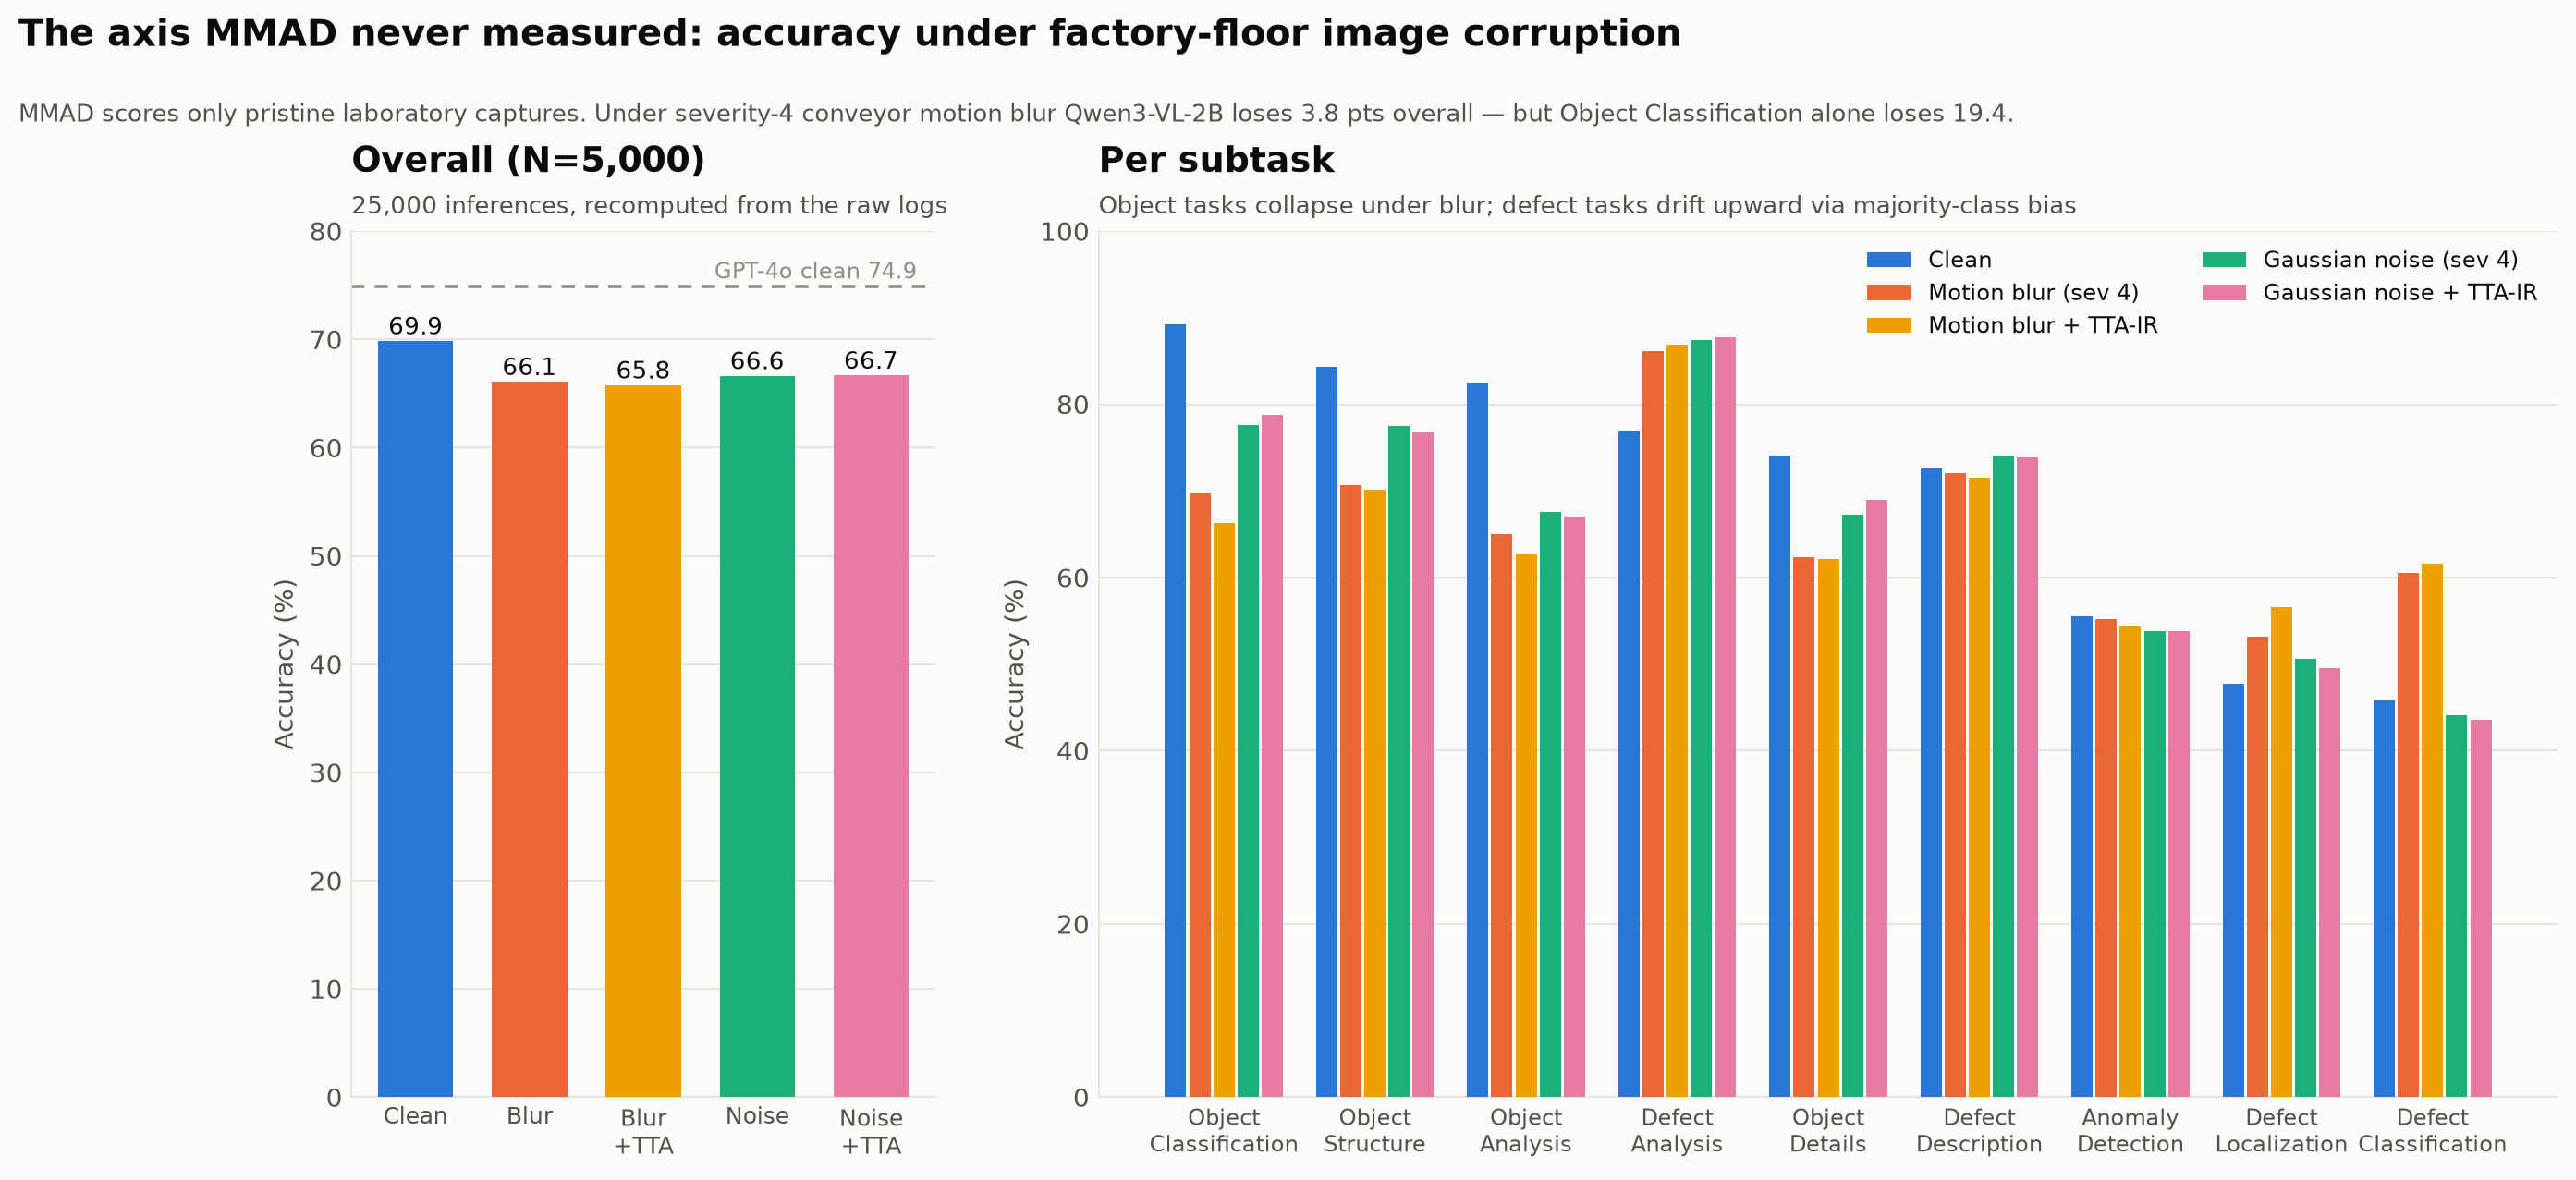
\includegraphics[width=0.85\textwidth]{fig6_robustness_gap.png}
\caption{Clean vs.\ corrupted vs.\ restored accuracy, overall and per subtask
(25{,}000 inferences). Object tasks collapse under motion blur; defect tasks drift
upward.}
\label{fig:robust}
\end{figure*}

\subsection{First \armB{} experiment (Phase 5)}\label{sec:armb}

\textbf{Pipeline.} A ResNet-50 PatchCore built a memory bank from up to eight normal
images per category, the heatmap was thresholded at a calibrated $\tau$, and the
resulting region was drawn as a red box with a ``DEFECT CANDIDATE'' tag
(Fig.~\ref{fig:vp}); the prompt told Qwen3-VL-2B to focus on the red region. If the
detector did not fire, the plain image and prompt were used.

\textbf{Result.} On 500 questions, guidance lowered accuracy from 72.2\,\% to
68.6\,\% ($-$3.6\pp). The paired comparison has 38 fixes and 56 breaks, exact
McNemar $p{=}0.079$: the drop is not significant, and neither is any per-subtask
change ($n{\approx}55$ per subtask, $\pm$13\pp). The pattern in
Fig.~\ref{fig:p5} is nonetheless suggestive: Defect Classification ($+$5.3\pp) and
Defect Analysis ($+$1.8\pp) improve, while Defect Localization ($-$10.9\pp) and
Object Analysis ($-$10.7\pp) degrade, consistent with a box that helps name a defect
but obscures the object and distorts coarse position judgements.

\textbf{Why this pilot cannot answer the question.} Auditing the run revealed three
problems:
\begin{enumerate}
  \item \emph{Mis-calibrated detector.} $\tau$ was estimated on normal images that
        were also in the memory bank, so it is biased low. The detector fired on
        92.6\,\% of all images, including normal ones: \armB{} was mostly
        ``box everywhere'', not detector guidance.
  \item \emph{Single-source sample.} All 500 questions came from GoodsAD (the other
        sources' normal-image folders did not resolve at the time).
  \item \emph{Silent parse fallback.} Unparseable outputs defaulted to ``A''.
\end{enumerate}
We therefore treat Phase~5 as a negative pilot that motivates the controlled design
below rather than as evidence against \armB.

\begin{figure}[t]
\centering
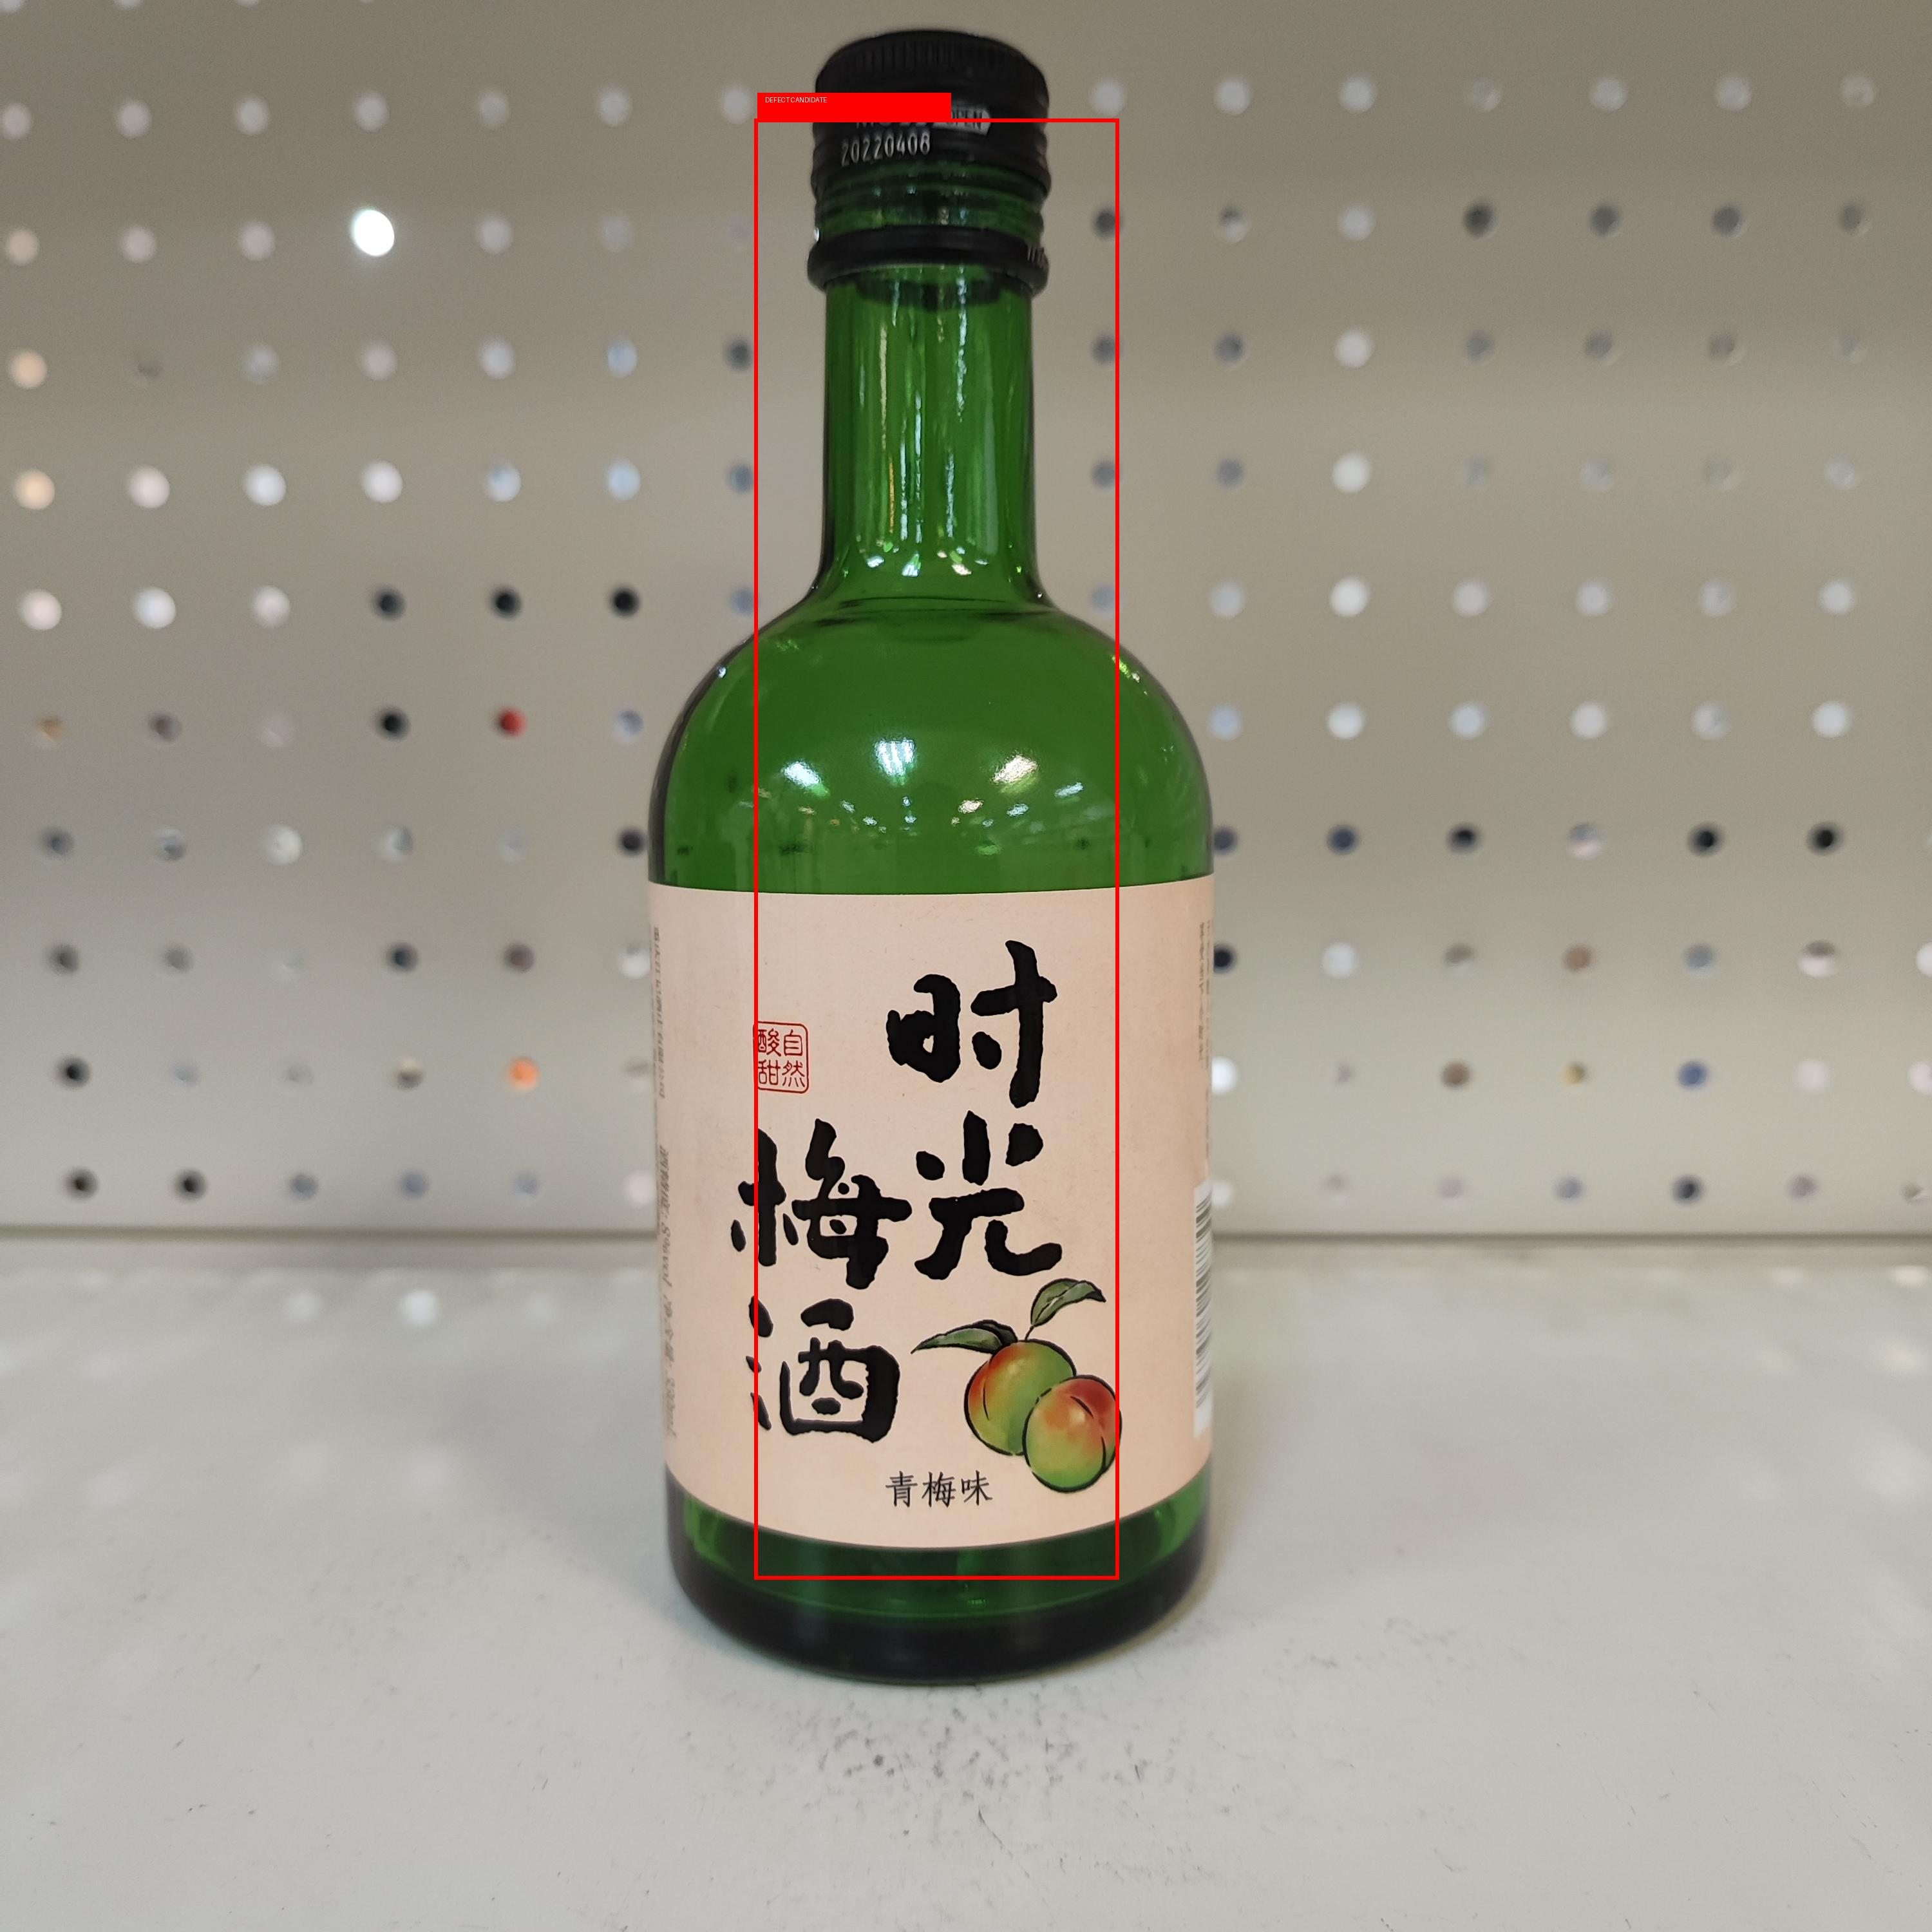
\includegraphics[width=0.62\columnwidth]{sample_visual_prompt.jpg}
\caption{Phase-5 visual prompt: PatchCore region drawn as a red box with a tag.}
\label{fig:vp}
\end{figure}

\begin{figure}[t]
\centering
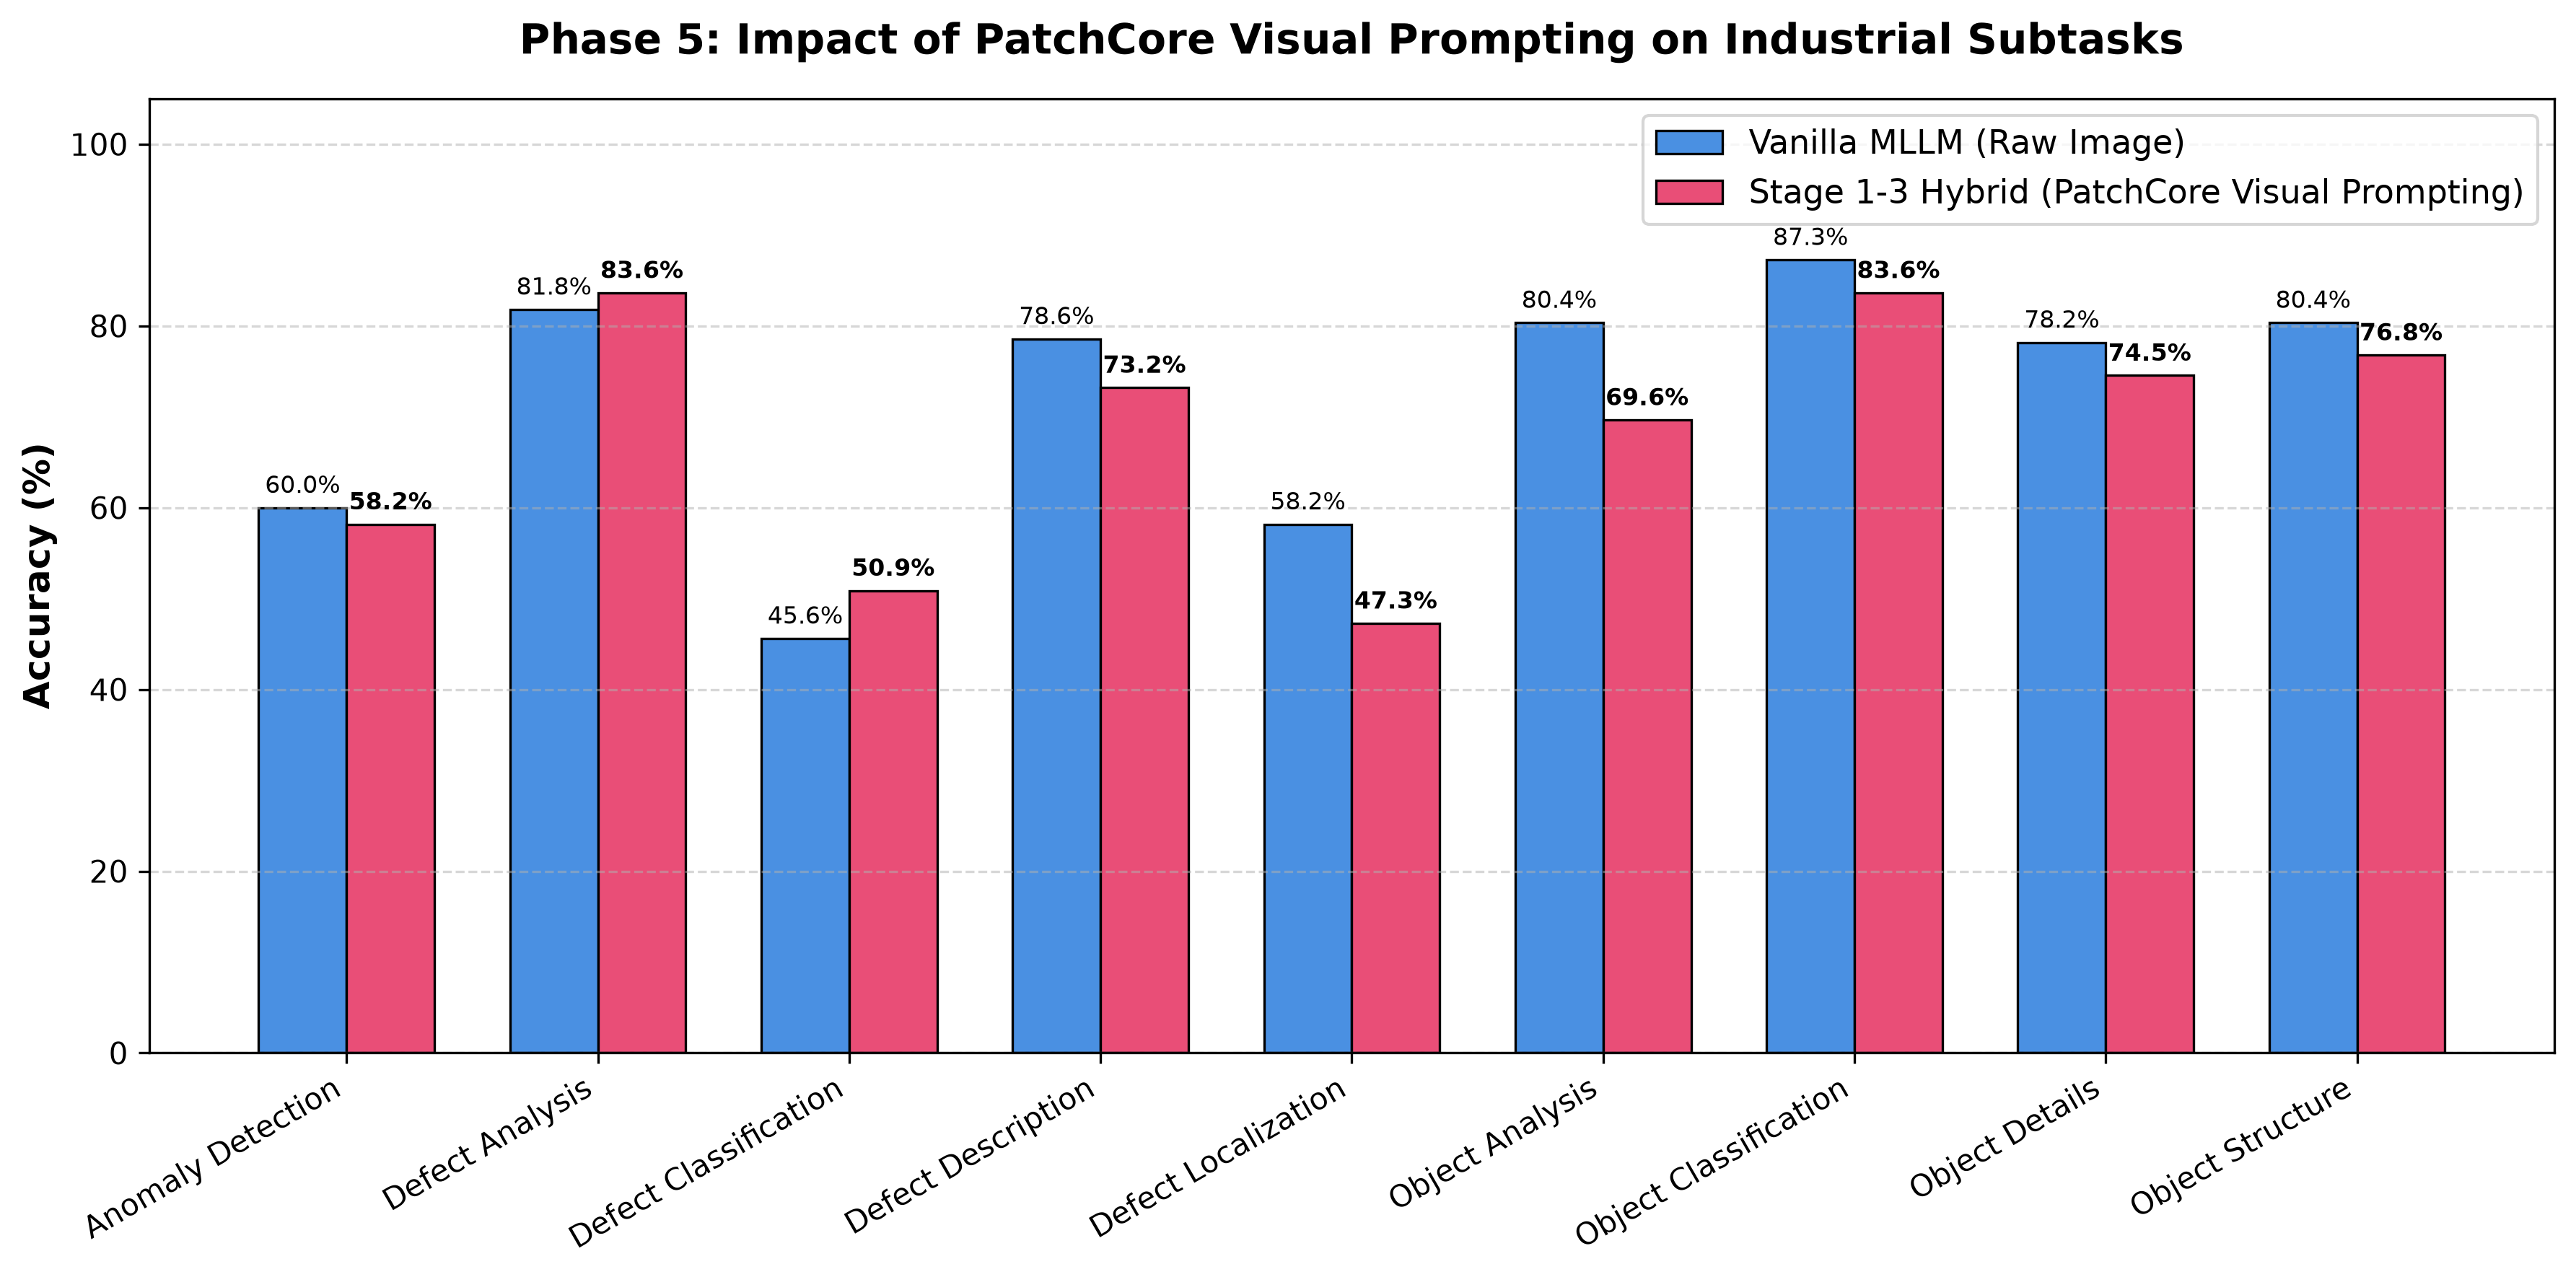
\includegraphics[width=\columnwidth]{phase5_subtask_delta.png}
\caption{Phase~5, \armA{} (blue) vs.\ PatchCore-guided \armB{} (red), 500 GoodsAD
questions. Overall $-$3.6\pp, McNemar $p{=}0.079$ (n.s.).}
\label{fig:p5}
\end{figure}

% =============================================================================
\section{Arm-B Lab: a research environment for detector-guided MLLMs}\label{sec:lab}

Answering whether detector guidance helps requires many controlled variants:
detectors of known quality, null controls, prompt styles, gating rules, models.
Writing a script per variant is what produced Phase~5's confounds, so we built
\emph{Arm-B Lab} (Fig.~\ref{fig:lab}): a local web application in the style of
ComfyUI, in which every block of Fig.~\ref{fig:pipeline} is a typed, swappable node.

\textbf{Architecture.} A FastAPI server hosts a node registry; each node declares
typed ports (\texttt{IMAGE}, \texttt{ANOMALY}, \texttt{REGION}, \texttt{QUESTION},
\texttt{RESPONSE}, \ldots) and widget parameters, and the browser builds its palette
from that schema. Graphs execute in topological order, and every node output is
cached under a fingerprint of (type, parameters, upstream fingerprints), so changing
a prompt re-runs only the prompt and the MLLM, and a sweep over a downstream
parameter runs the detector once per image. A single worker queue serialises GPU
work.

\textbf{Nodes.} Table~\ref{tab:nodes} lists the node families. Three are designed
specifically as experimental controls: a \emph{synthetic detector} built from the
ground-truth mask with adjustable miss rate, false-alarm rate, shift and dilation
(with defaults it is an oracle, giving the ceiling of \armB); a \emph{control
detector} that draws a random box, a centre box or the whole image (does \emph{any}
box help?); and a \emph{selective gate} that applies guidance only to chosen
subtasks, the recommendation that followed from Phase~5.

\textbf{Evaluation.} A batch run takes a stratified MMAD sample and an optional grid
of parameter values. Every variant sees the same questions, so arms and variants are
compared with paired statistics: accuracy with Wilson intervals, $\kappa$, macro
accuracy, parse-failure rate, exact McNemar with fixes/breaks, accuracy conditioned
on whether the detector fired, RDS and spread across sweep values, and, in
letter-logit mode, expected calibration error~\cite{guo2017calibration}. Detector
nodes are scored against ground-truth masks (image AUROC on $\tau$-normalised
scores and per category, pixel AUROC, box IoU, gate TPR/FPR). Runs are logged per
question as JSONL, are resumable, and export 300-dpi figures and a manifest.

\textbf{Fixes relative to Phase 5.} $\tau$ is calibrated on held-out normal images
never placed in the memory bank; normal references come from MMAD's own template
lists (query image excluded) for all five sources; parse failures are counted as
wrong unless the Phase-5 fallback is explicitly selected for reproduction.

\textbf{Implementation checks.} PatchCore follows~\cite{roth2022patchcore} (greedy
coreset on a random projection, local 3$\times$3 aggregation, configurable backbone
and layers). WinCLIP is re-implemented with true window masking on OpenAI
ViT-B/16. A first version mixed CLIP's last-layer patch tokens into the zero-shot map
and produced \emph{inverted} maps (pixel AUROC 0.27), consistent with the known
misalignment of those tokens~\cite{li2023clipsurgery}; the corrected version uses
window embeddings only for zero-shot and penultimate-layer tokens for the few-shot
memory. On a 24-image check (Table~\ref{tab:detpilot}) the expected ordering
PatchCore $>$ WinCLIP+ $>$ WinCLIP zero-shot holds. On the GPU, Qwen3-VL-2B answers
in 0.17\,s per question (4.5\,GB) in generation mode and 0.18\,s in letter-logit mode.

\begin{table}[t]
\centering
\caption{Arm-B Lab node families.}
\label{tab:nodes}
\footnotesize
\begin{tabular}{@{}p{1.5cm}p{6.5cm}@{}}
\toprule
Family & Nodes (key parameters) \\
\midrule
Input & MMAD sample (source, subtask, defective/normal); normal references ($k$, template strategy); own image / question \\
Pre-process & Corruption engine (7$\times$5); test-time restoration \\
Question & Question builder (3 paraphrases, option shuffling) \\
Detector & PatchCore (backbone, layers, resolution, coreset, $k$-NN, $\tau$ margin); WinCLIP / WinCLIP+ (CLIP model, scales, templates); synthetic GT detector; null control \\
Localise & Heatmap$\rightarrow$box (gate: calibrated/fixed/always/never; threshold: calibrated/relative/percentile/Otsu) \\
Prompt & Visual prompt (9 styles: box, box+wash, contour, heatmap, crop, side-by-side, blur/darken outside); text prompt (7 templates incl.\ hedged hint); selective gate \\
Reason & MLLM (any local Qwen/SmolVLM/Gemma, precision, generate vs.\ letter-logits, temperature, seed) \\
Evaluate & Answer parser (strict/lenient/tag); score; detector metrics \\
\bottomrule
\end{tabular}
\end{table}

\begin{table}[t]
\centering
\caption{Detector sanity check in the lab (24 VisA/DS-MVTec images, 12 defective,
$k{=}8$ normal references; image AUROC on raw scores pooled across categories).
Preliminary --- to be replaced by the full detector benchmark (E3).}
\label{tab:detpilot}
\footnotesize
\begin{tabular}{@{}lrr@{}}
\toprule
Detector & Image AUROC & Pixel AUROC \\
\midrule
PatchCore (WRN-50, layer2+3) & 0.861 & 0.923 \\
WinCLIP+ (few-shot, $k{=}8$) & 0.833 & 0.825 \\
WinCLIP (zero-shot)          & 0.792 & 0.684 \\
\bottomrule
\end{tabular}
\end{table}

\begin{figure*}[t]
\centering
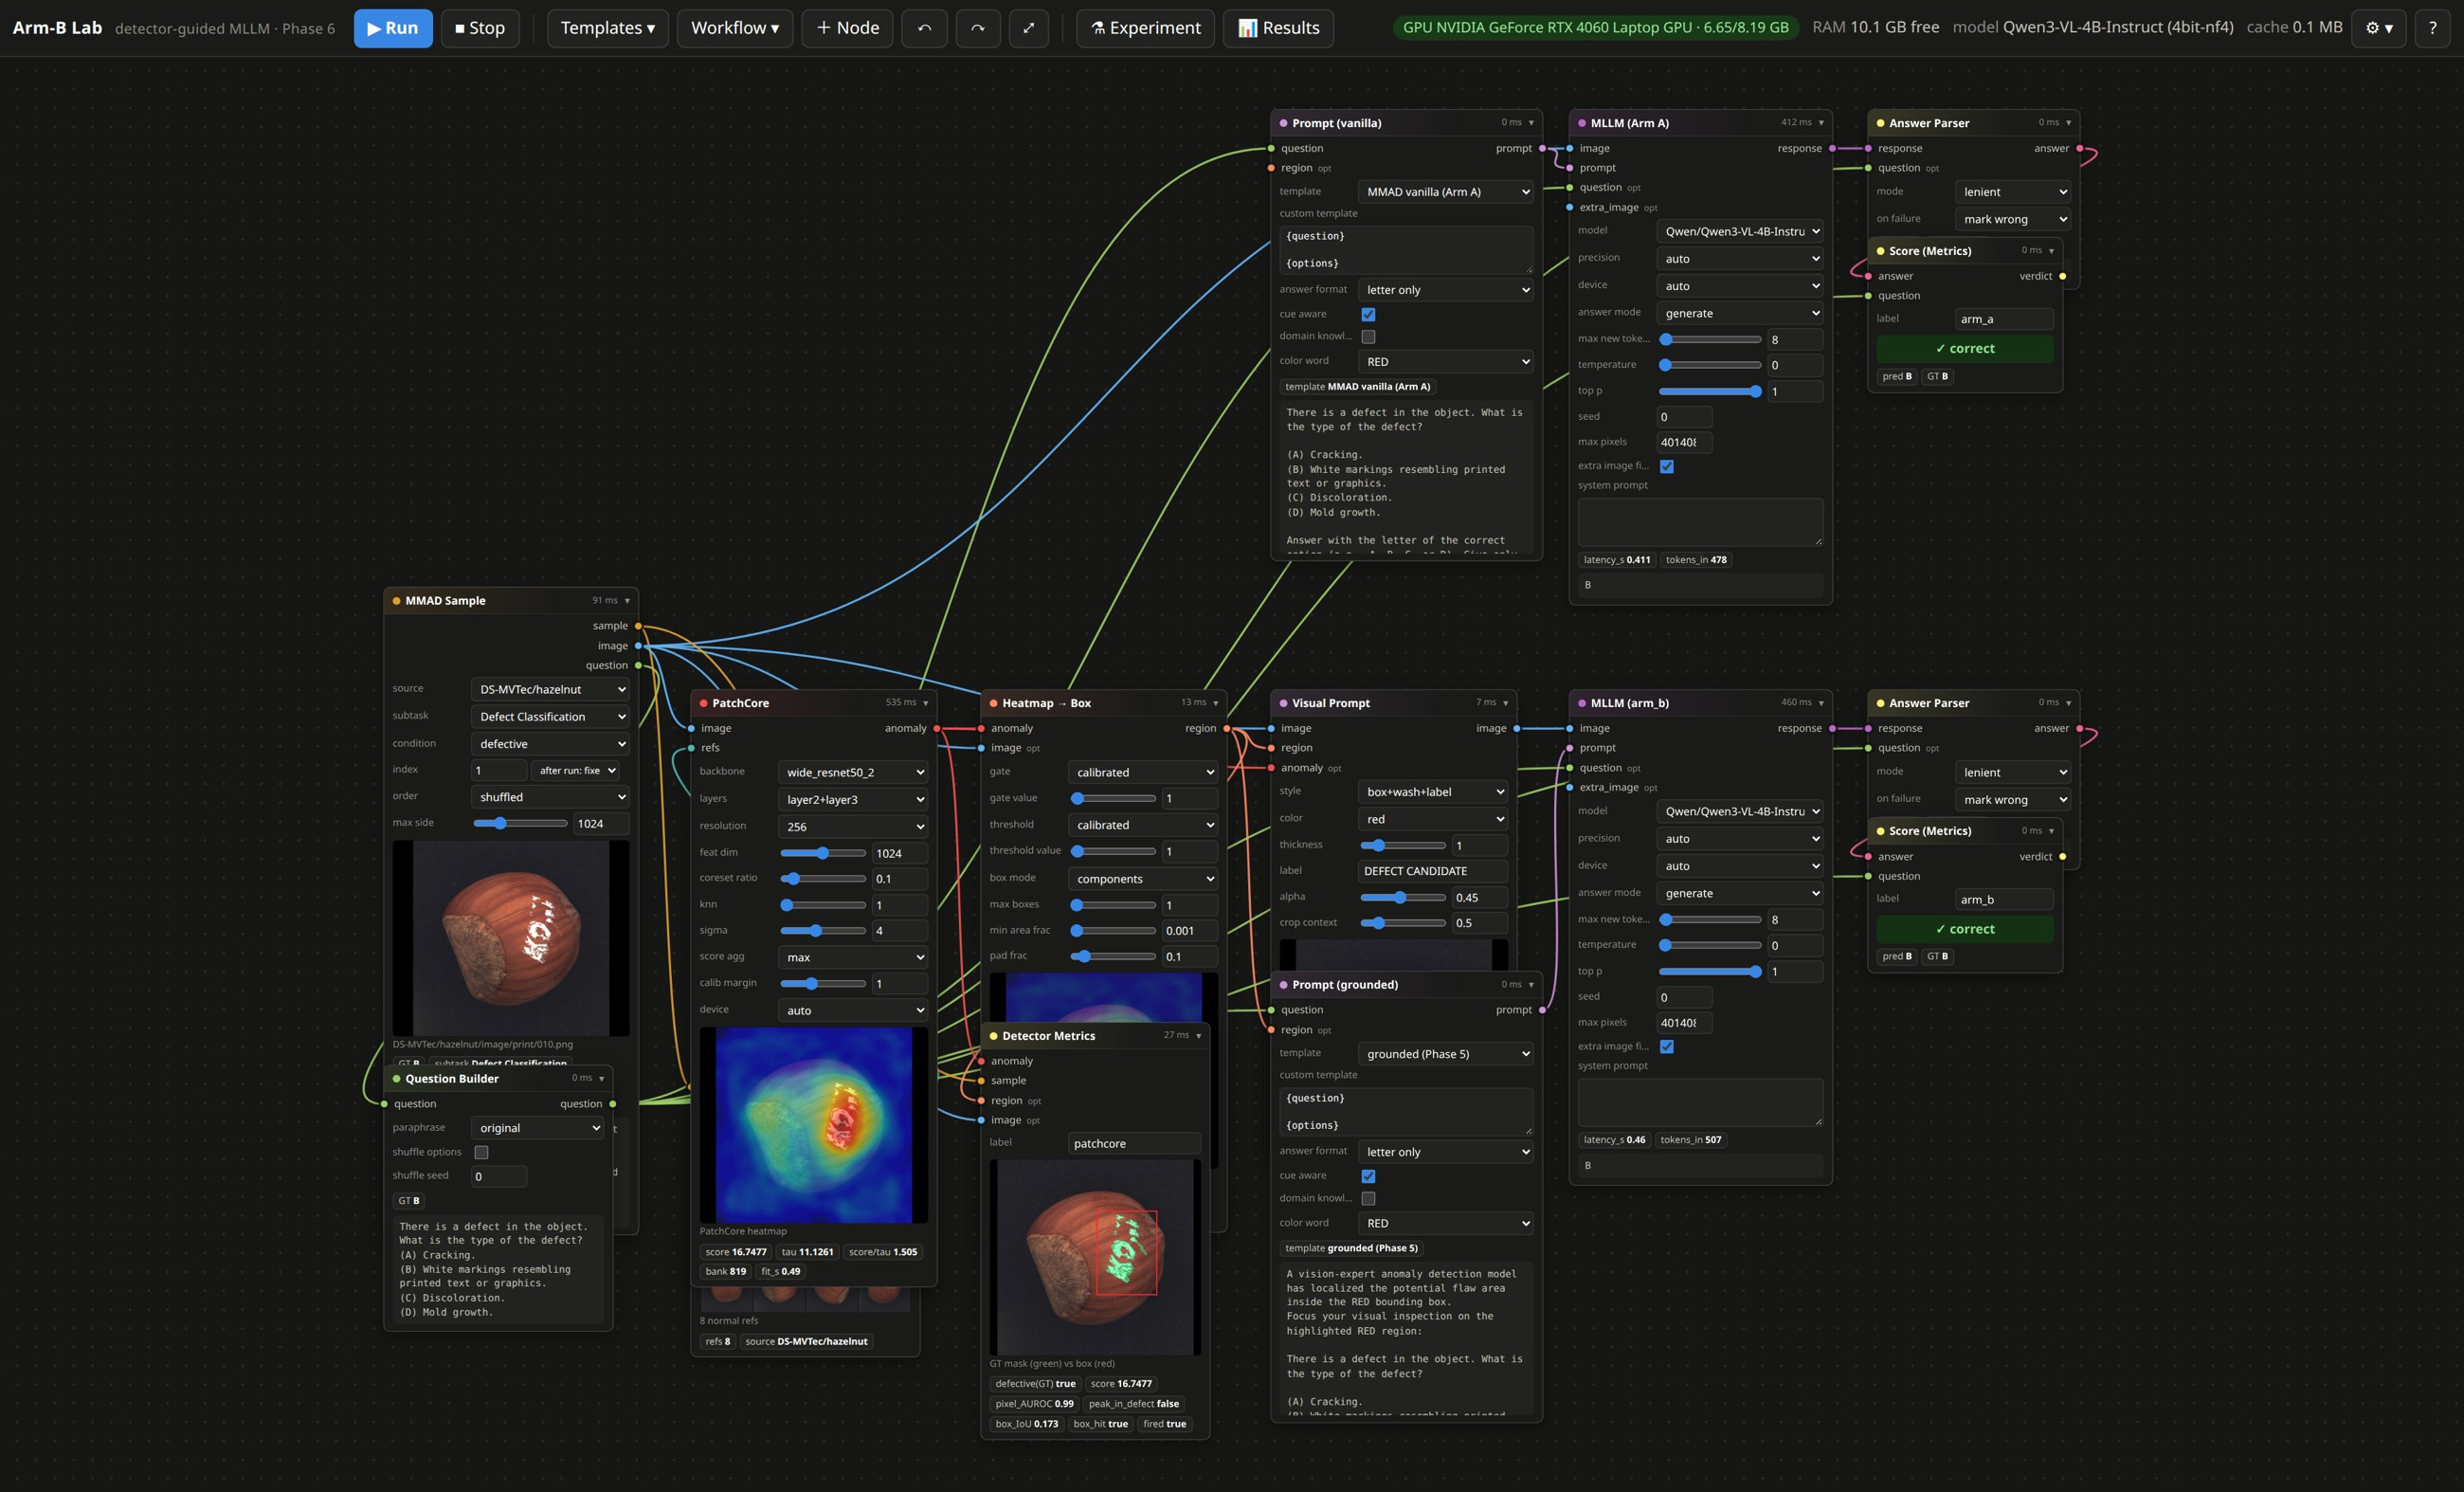
\includegraphics[width=\textwidth]{lab_editor_arm_a_vs_b.jpg}
\caption{Arm-B Lab running the paired \armA{} (top row) vs.\ \armB{} (bottom row)
graph on an MMAD hazelnut ``print'' defect with Qwen3-VL-4B (NF4). Each node shows its
output: PatchCore heatmap ($\text{score}/\tau{=}1.51$), the box drawn for the MLLM,
the ground-truth mask vs.\ box (pixel AUROC 0.99, box IoU 0.17), the prompts and
both verdicts. Right-click replaces PatchCore by WinCLIP or a control detector
while keeping the wiring.}
\label{fig:lab}
\end{figure*}

% =============================================================================
\section{Discussion}

\subsection{What the completed phases show}

(i) A 2\,B open model on a laptop GPU is a credible zero-shot inspector on MMAD's
question types, within about 6.5 points of GPT-4o's 1-shot average; (ii) the weak
spots are fine-grained defect classification and localisation, exactly where a
pixel-level detector should help; (iii) aggregate accuracy understates corruption
damage, and training-free restoration does not repair it; (iv) naive
detector-guided prompting did not help, but the only test of it was confounded.

\subsection{Threats to validity}

\emph{Shot setting}: our zero-shot numbers are compared with MMAD's 1-shot table.
\emph{Sample size}: 2{,}500 of 39{,}672 questions; per-subtask differences under
$\sim$6\pp{} are not resolvable. \emph{Question sets}: Phase~1 and Phase~4 draws
differ slightly. \emph{Quantisation}: 8B, 4B and Gemma-4-E4B ran in NF4, the others
in FP16, so architecture and precision are confounded. \emph{Model vintage}: our
models are one to two years newer than the paper's. \emph{Label inference}: the
normal/abnormal split for balanced accuracy is inferred from the \texttt{/good/}
path convention. \emph{Single seed}: all runs are greedy with one sampling seed.

\subsection{Consistency audit of the earlier manuscript}

Recomputing every table from the raw logs showed that 28 of 36 per-subtask cells in
the earlier thesis draft disagree with the artefacts by more than 0.5 points. The
draft's ``Phase~1'' table matches the clean column of the 5{,}000-question study
(mean absolute difference 0.08) rather than the Phase-1 run (3.62), i.e.\ it is
correct data under the wrong label; the cross-model subtask table diverges by up to
11.7 points and must be regenerated. All numbers in this draft come from the
artefacts.

% =============================================================================
\section{Remaining Work}\label{sec:roadmap}

Table~\ref{tab:roadmap} lists the experiments planned with Arm-B Lab. Each is paired
(same questions across arms) and uses all five MMAD sources. At $N{=}1{,}800$
(200 per subtask) the overall 95\,\% half-width is about $\pm$2.1\pp; paired McNemar
tests are more sensitive than that. With Qwen3-VL-2B at $\sim$0.2\,s per question,
the MLLM cost of one arm at $N{=}1{,}800$ is about six minutes.

\begin{table*}[t]
\centering
\caption{Planned experiments (all runnable as saved Arm-B Lab templates).}
\label{tab:roadmap}
\footnotesize
\begin{tabular}{@{}p{0.6cm}p{4.3cm}p{6.2cm}p{4.9cm}@{}}
\toprule
ID & Experiment & Question it answers & Design \\
\midrule
E1 & \armA{} vs.\ calibrated PatchCore \armB & Does detector guidance help once the detector is calibrated and data are balanced? & $N{=}1{,}800$, 5 sources, McNemar, acc.\ conditioned on detector firing \\
E2 & Oracle / random box / no box & Ceiling of \armB; does \emph{any} box help? & Synthetic GT detector vs.\ control detector vs.\ \armA, defective images \\
E3 & Detector benchmark & PatchCore vs.\ WinCLIP(+) quality on MMAD images & Image/pixel AUROC, IoU, gate TPR/FPR, one row per image \\
E4 & Detector-quality sweep & How good must the detector be? & Sweep synthetic miss rate, false-alarm rate and shift \\
E5 & Gate \& threshold sweep & Precision/recall trade-off of firing & Sweep gate value and box threshold \\
E6 & Visual-prompt style & Box vs.\ contour vs.\ crop vs.\ heatmap vs.\ blur-outside & Same detector, paired across styles \\
E7 & Text prompt / trust & Does a hedged hint avoid the harm of false boxes? & Grounded vs.\ hedged vs.\ score-annotated prompts \\
E8 & Selective gating & Guide only Defect Classification/Analysis? & Gated vs.\ always-guided vs.\ \armA \\
E9 & Robust \armB & Does the detector help or fail under corruption? & Severity 0--5 sweep on both arms, RDS per arm \\
E10 & Prompt sensitivity & Paraphrase spread, letter-position bias & 4 paraphrases $\times$ option shuffling \\
E11 & Calibration & Are confident answers correct? & Letter-logit probabilities, ECE, reliability diagrams \\
E12 & Model scaling of \armB & Does guidance matter less for 8B than for 2B? & Qwen3-VL 2B/4B/8B, Moondream2, Gemma-4 \\
E13 & Official protocol & Full-benchmark, 1-shot numbers & MMAD code on all 8{,}366 images incl.\ GoodsAD \\
E14 & Repeatability & Seed and run-to-run variance & 3 sampling seeds for the headline comparisons \\
\bottomrule
\end{tabular}
\end{table*}

Writing tasks: regenerate the manuscript tables from the manifests; replace
Phase~2's small severity sweep by E9 at scale; confirm the majority-class
interpretation of the corruption results with confusion matrices; verify the
\texttt{TODO}-marked references.

% =============================================================================
\section{Conclusion}

Small open MLLMs running on a single laptop GPU already answer industrial-inspection
questions at a level close to large commercial models, but they are weakest at
naming and locating defects and are fragile to motion blur in ways that aggregate
accuracy hides. Our first attempt at detector guidance did not help, for reasons we
can now identify and control. Arm-B Lab turns the remaining question, when a
classical anomaly detector helps a small MLLM and when it misleads it, into a set of
paired, reproducible experiments, which form the next stage of this work.

\section*{Reproducibility}
Code, run logs and figures are in the \texttt{Open-IAD} repository: phases 0--5 under
\texttt{Local-training/phase-*}, the recomputed comparison under
\texttt{comparative-analysis/}, and Arm-B Lab under \texttt{Local-training/phase-6}
(\texttt{./run\_lab.sh}).

\bibliographystyle{IEEEtran}
\bibliography{refs}

\end{document}
